\documentclass[12pt,a4paper]{article}

% ---------- Packages ----------
\usepackage[T1]{fontenc}
\usepackage{mathptmx}
\usepackage[
    top=1.15in,
    bottom=1.1in,
    left=1.15in,
    right=1.15in,
    headheight=18pt,
    headsep=0.45in,
    footskip=0.45in
]{geometry}

\usepackage{graphicx}
\usepackage{tikz}
\usetikzlibrary{positioning,arrows.meta,shapes.geometric,shapes.multipart,fit,calc}
\usepackage{setspace}
\usepackage{ragged2e}
\usepackage{tabularx}
\usepackage{array}
\usepackage{booktabs}
\usepackage{float}
\usepackage{enumitem}
\usepackage{xcolor}
\usepackage{fancyhdr}
\usepackage{needspace}
\usepackage{longtable}
\usepackage{listings}
\usepackage{caption}

% Code Listing Configuration
\definecolor{codebg}{rgb}{0.97,0.97,0.97}
\definecolor{codekeyword}{rgb}{0.0,0.2,0.6}
\definecolor{codecomment}{rgb}{0.2,0.5,0.2}
\definecolor{codestring}{rgb}{0.7,0.1,0.1}

\lstdefinelanguage{JavaScript}{
  keywords={typeof, new, true, false, catch, function, return, null, switch, var, if, in, while, do, else, case, break, const, let, useEffect, useState, fetch, async, await},
  ndkeywords={class, export, boolean, throw, implements, import, this},
  sensitive=true,
  comment=[l]{//},
  morecomment=[s]{/*}{*/},
  morestring=[b]',
  morestring=[b]"
}

\lstdefinestyle{cleanstyle}{
    backgroundcolor=\color{codebg},
    commentstyle=\color{codecomment}\itshape,
    keywordstyle=\color{codekeyword}\bfseries,
    numberstyle=\tiny\color{gray},
    stringstyle=\color{codestring},
    basicstyle=\ttfamily\footnotesize,
    breaklines=true,
    breakatwhitespace=false,
    captionpos=b,
    numbers=left,
    numbersep=6pt,
    tabsize=2,
    showstringspaces=false
}
\lstset{style=cleanstyle}
\captionsetup{font=small,labelfont=bf,skip=6pt}


% ---------- General formatting ----------
\pagestyle{empty}
\setlength{\parindent}{0pt}

\newcommand{\tbd}[1]{\textcolor{red}{\textbf{[#1]}}}

% ---------- Page border ----------
\newcommand{\pageborder}{%
  
\begin{tikzpicture}[remember picture,overlay]
    \draw[line width=2pt]
      ([xshift=0.9in,yshift=-0.9in]current page.north west)
      rectangle
      ([xshift=-0.9in,yshift=0.9in]current page.south east);
  \end{tikzpicture}%
}

% ---------- Header and footer: Table of Contents ----------
\fancypagestyle{toc}{%
  \fancyhf{}
  \fancyhead[L]{\large\bfseries\itshape InterfaceGuard\pageborder}
  \fancyhead[R]{}
  \fancyfoot[L]{\large\itshape Department of Computer Applications -- ASIET}
  \fancyfoot[R]{}
  \renewcommand{\headrulewidth}{0pt}
  \renewcommand{\footrulewidth}{0pt}
}

% ---------- Header and footer: Report body ----------
\fancypagestyle{reportbody}{%
  \fancyhf{}
  \fancyhead[L]{\large\bfseries\itshape InterfaceGuard\pageborder}
  \fancyhead[R]{}
  \fancyfoot[L]{\large\itshape Department of Computer Applications -- ASIET}
  \fancyfoot[R]{\large\bfseries\thepage}
  \renewcommand{\headrulewidth}{0pt}
  \renewcommand{\footrulewidth}{0pt}
}

% ---------- Header and footer: Chapter opening pages ----------
\fancypagestyle{plain}{%
  \fancyhf{}
  \fancyhead[L]{\large\bfseries\itshape InterfaceGuard\pageborder}
  \fancyhead[R]{}
  \fancyfoot[L]{\large\itshape Department of Computer Applications -- ASIET}
  \fancyfoot[R]{\large\bfseries\thepage}
  \renewcommand{\headrulewidth}{0pt}
  \renewcommand{\footrulewidth}{0pt}
}

% ---------- College logo ----------
\newcommand{\collegelogo}[1]{%
  \IfFileExists{logo.png}
    {\includegraphics[width=#1]{logo.png}}
    {\fbox{\parbox[c][#1][c]{#1}{\centering\small College Logo}}}%
}

% ---------- Table column definitions ----------
\newcolumntype{C}[1]{>{\centering\arraybackslash}m{#1}}
\newcolumntype{L}[1]{>{\raggedright\arraybackslash}p{#1}}
\newcolumntype{M}{>{\raggedright\arraybackslash}m{\dimexpr\linewidth-1.8cm-2.4cm-6\tabcolsep-4\arrayrulewidth\relax}}
\newcolumntype{Y}{>{\raggedright\arraybackslash}X}

% ---------- General formatting ----------
\pagestyle{empty}
\setlength{\parindent}{0pt}
\setlength{\emergencystretch}{3em}
\setlength{\tabcolsep}{5pt}

\begin{document}
\pagenumbering{roman}

% ============================================================
% TITLE PAGE
% ============================================================
\pageborder

\begin{center}
\vspace*{0.1in}

{\large\bfseries
INTERFACEGUARD: AN AI-ASSISTED TOOL FOR DETECTING\\
OBJECT-ORIENTED INTERFACE EROSION}\\[10pt]

{\normalsize A PROJECT REPORT}\\[4pt]
{\small Submitted by}\\[22pt]

{\large\bfseries ATHUL KRISHNA}\\[8pt]
{\large\bfseries ASI25MCA-2020}\\[22pt]

{\small\bfseries Under the Guidance of}\\[4pt]
{\large\bfseries Ms. RINTU AUGUSTINE}\\[4pt]
{\footnotesize\bfseries Associate Professor}\\[24pt]

to\\[4pt]
{\small the APJ Abdul Kalam Technological University}\\[2pt]
{\small in partial fulfillment of the requirements for the award of the Degree}\\[2pt]
of\\[2pt]
{\small\itshape Master of Computer Applications}\\[28pt]

\collegelogo{1.6in}\\[28pt]

{\large\bfseries Department Of Computer Applications}\\[6pt]
{\normalsize Adi Shankara Institute of Engineering \& Technology}\\[4pt]
{\normalsize Mattoor, Kalady Ernakulam District, Kerala State}\\[4pt]
{\normalsize Pin:683574}\\[8pt]
{\normalsize October, 2026}

\end{center}

\newpage

% ============================================================
% DECLARATION
% ============================================================
\pageborder
\vspace*{0.5in}

\begin{center}
{\large\bfseries DECLARATION}
\end{center}

\vspace{0.2in}

\begin{spacing}{1.5}
\justifying
I undersigned, hereby declare that the project report
``INTERFACEGUARD: AN AI-ASSISTED TOOL FOR DETECTING OBJECT-ORIENTED
INTERFACE EROSION'' submitted for partial fulfilment of the
requirements for the award of degree of Master of Computer Applications
of the APJ Abdul Kalam Technological University, Kerala is a Bonafide
work done by me under supervision of Ms. Rintu Augustine. This submission
represents my ideas in my own words and where ideas or words of others
have been included, I have adequately and accurately cited and referenced
the original sources. I also declare that I have adhered to ethics of
academic honesty and integrity and have not misrepresented or fabricated
any data or idea or fact or source in my submission. I understand that
any violation of the above will be a cause for disciplinary action by
the institute and/or the University and can also evoke penal action from
the sources which have thus not been properly cited or from whom proper
permission has not been obtained. This report has not been previously
formed the basis for the award of any degree, diploma or similar title
of any other University.
\end{spacing}

\vspace{0.5in}

\noindent Place : KALADY \hfill Signature\\[2pt]
Date : \hfill \textbf{ATHUL KRISHNA}

\newpage

% ============================================================
% CERTIFICATE
% ============================================================
\pageborder

\begin{center}
\vspace*{0.1in}

{\large\bfseries
ADI SHANKARA INSTITUTE OF ENGINEERING AND\\
TECHNOLOGY}\\[6pt]

{\large\bfseries VIDYA BHARATHI NAGAR, MATTOOR, KALADY}\\[6pt]
{\large\bfseries DEPARTMENT OF COMPUTER APPLICATIONS}\\[14pt]

\collegelogo{1.6in}\\[30pt]

{\large\bfseries CERTIFICATE}
\end{center}

\vspace{0.2in}

\begin{spacing}{1.5}
\noindent
\begin{minipage}{0.98\textwidth}
\justifying
This is to certify that the report entitled
``{\large\bfseries INTERFACEGUARD: AN AI-ASSISTED TOOL FOR DETECTING
OBJECT-ORIENTED INTERFACE EROSION}'' submitted by
\textbf{ATHUL KRISHNA} to the APJ Abdul Kalam Technological University
in partial fulfillment of the requirements for the award of the Degree
of Master of Computer Applications, is a Bonafide record of the project
work carried out by him under my guidance and supervision. This report
in any form has not been submitted to any other University or Institute
for any purpose.
\end{minipage}
\end{spacing}

\vspace{0.9in}

\noindent
\begin{minipage}[t]{0.48\textwidth}
\centering
Ms. Rintu Augustine\\
Project Guide\\
Department of Computer Applications
\end{minipage}
\hfill
\begin{minipage}[t]{0.48\textwidth}
\centering
Dr. Vincy Devi V K\\
Head of the Department\\
Department of Computer Applications
\end{minipage}

\newpage

% ============================================================
% ACKNOWLEDGEMENT
% ============================================================
\pageborder
\vspace*{0.3in}

\begin{center}
{\large\bfseries ACKNOWLEDGEMENT}
\end{center}

\vspace{0.1in}

\begin{spacing}{1.5}
\justifying
I am profoundly grateful for the support and guidance that have been
instrumental in the successful completion of this project, InterfaceGuard:
An AI-Assisted Tool for Detecting Object-Oriented Interface Erosion.

First and foremost, I extend my heartfelt thanks to Ms. Rintu Augustine,
Associate Professor, whose invaluable guidance, mentorship, and constructive
feedback have been instrumental throughout this project. Her encouragement
and direction helped shape this work into a practical tool that supports
developers in understanding and maintaining the design quality of their
software. I would also like to express my sincere appreciation to
Dr. Vincy Devi V K, Head of the Department, for her constant encouragement
and for fostering an environment that promotes innovation and research-driven
learning.

I am equally thankful to ADI SHANKARA INSTITUTE OF ENGINEERING AND TECHNOLOGY
for providing the resources, infrastructure, and learning environment that
enabled me to delve deeply into this complex and rewarding field. The access
to advanced tools and a supportive community has significantly enriched
my experience.

Lastly, I want to acknowledge the open-source community and various online
forums for their rich repositories of knowledge, tools, and technical
discussions, which served as critical references throughout the development
process.
\end{spacing}

\vspace{0.3in}
\noindent\textbf{ATHUL KRISHNA}

\newpage

% ============================================================
% ABSTRACT
% ============================================================
\pageborder
\vspace*{0.3in}

\begin{center}
{\large\bfseries ABSTRACT}
\end{center}

\vspace{0.1in}

\begin{spacing}{1.5}
\justifying
This project, titled ``INTERFACEGUARD: AN AI-ASSISTED TOOL FOR DETECTING
OBJECT-ORIENTED INTERFACE EROSION,'' addresses a common maintainability
problem in object-oriented software. As a system evolves through repeated
changes, its interfaces gradually accumulate unrelated responsibilities,
a decay known as interface erosion. It shows up as bloated interfaces,
violations of the Interface Segregation Principle, cyclic dependencies,
rising coupling, and implementing classes forced to write empty or unused
methods. Existing free static analysis tools report metrics and code smells
only at a single point in time, and they neither reveal when a design began
to degrade nor explain the problem to the developer in plain language.
InterfaceGuard imports a Java repository from a public GitHub URL, parses
it with JavaParser, and mines its commit history with PyDriller. For every
interface it computes Chidamber--Kemerer metrics together with erosion
metrics such as method-count growth, churn, breaking changes and interface
cohesion, and it detects Interface Segregation Principle violations,
dependency cycles and common code smells. These indicators are combined
into an Interface Health Score for each interface and an Erosion Index for
the whole project, and change-point detection is applied to the score
history to locate the commit at which an interface begins to erode. A
free-tier Large Language Model API then produces a plain-language
explanation and a refactoring recommendation for each flagged interface.
The results are presented on an interactive web dashboard built with a
Flask backend, a React frontend and a SQLite database, with dependency
graphs, trend charts and a downloadable PDF report. By relying entirely
on free and open-source components, InterfaceGuard offers students and
small development teams a practical, history-aware way to notice, locate
and understand interface erosion early, and it also serves as a teaching
aid for good object-oriented design.
\end{spacing}

\newpage

% ============================================================
% TABLE OF CONTENTS
% ============================================================
\pagestyle{toc}

% ---------- TOC PAGE 1 ----------
\begin{center}
{\large\bfseries TABLE OF CONTENTS}
\end{center}

\vspace{4pt}

\renewcommand{\arraystretch}{1.75}
\noindent\begin{tabular}{|C{1.8cm}|M|C{2.4cm}|}
\hline
\textbf{Sl. No.} & \textbf{Content} & \textbf{Page No.} \\
\hline
\textbf{1} & \textbf{INTRODUCTION} & \textbf{1--7} \\
\hline
1.1 & Brief introduction about the project & 1 \\
\hline
1.2 & Project Background & 2 \\
\hline
1.3 & Existing System & 2 \\
\hline
1.4 & Proposed System & 3 \\
\hline
1.5 & Basic Design principle of the project & 4 \\
\hline
1.6 & Basic Architecture of the project & 6 \\
\hline
\textbf{2} & \textbf{SYSTEM STUDY AND ANALYSIS} & \textbf{9--19} \\
\hline
2.1 & Drawbacks of the Existing System & 9 \\
\hline
2.2 & Problem Statement & 10 \\
\hline
2.3 & Feasibility Study & 11 \\
\hline
2.4 & Project Planning & 13 \\
\hline
2.5 & Requirement Specification & 15 \\
\hline
\textbf{3} & \textbf{SYSTEM WORK FLOW} & \textbf{16} \\
\hline
3.1 & Design Methodology & 16 \\
\hline
3.2 & UML diagrams & 18 \\
\hline
3.3 & Use case design & 19 \\
\hline
\textbf{4} & \textbf{AGILE TECHNOLOGY OVERVIEW} & \textbf{20--26} \\
\hline
4.1 & Introduction to Scrum & 20 \\
\hline
4.2 & Principles or methodology used & 21 \\
\hline
4.3 & Product Backlog & 22 \\
\hline
4.4 & Sprint Planner & 23 \\
\hline
4.5 & Ideal Burn down chart & 23 \\
\hline
\end{tabular}

\newpage

% ---------- TOC PAGE 2 ----------
\vspace*{0.1in}

\renewcommand{\arraystretch}{1.75}
\noindent\begin{tabular}{|C{1.8cm}|M|C{2.4cm}|}
\hline
\textbf{5} & \textbf{SYSTEM DESIGN} & \textbf{27--30} \\
\hline
5.1 & Technology / framework [MVC] & 27 \\
\hline
5.2 & Module Description & 29 \\
\hline
\textbf{6} & \textbf{CODING} & \textbf{31--38} \\
\hline
6.1 & Coding standards used in the project & 31 \\
\hline
6.2 & Project coding & 34 \\
\hline
\textbf{7} & \textbf{TESTING} & \textbf{39--40} \\
\hline
7.1 & Unit Testing & 39 \\
\hline
\textbf{8} & \textbf{IMPLEMENTATION} & \textbf{41--43} \\
\hline
8.1 & Implementation method used in Project & 41 \\
\hline
\textbf{9} & \textbf{BUSINESS PERSPECTIVE} & \textbf{44--46} \\
\hline
\textbf{10} & \textbf{FUTURE SCOPE OR ENHANCEMENTS} & \textbf{47--49} \\
\hline
\textbf{11} & \textbf{APPENDIX} & \textbf{50--54} \\
\hline
11.1 & Git History [sprint wise] & 50 \\
\hline
11.2 & Screen Shots of Forms, Reports, Diagrams & 52 \\
\hline
11.3 & Burn down charts & 54 \\
\hline
\textbf{12} & \textbf{REFERENCES/BIBLIOGRAPHY} & \textbf{55--56} \\
\hline
\end{tabular}

\clearpage

% ============================================================
% ACTIVATE REPORT BODY AND START ARABIC PAGE 1
% ============================================================
\pagestyle{reportbody}
\pagenumbering{arabic}
\setcounter{page}{1}

\renewcommand{\thesection}{\arabic{section}.}
\renewcommand{\thesubsection}{\arabic{section}.\arabic{subsection}}
\renewcommand{\thesubsubsection}{%
  \arabic{section}.\arabic{subsection}.\arabic{subsubsection}%
}

% ============================================================
% CHAPTER 1: INTRODUCTION
% ============================================================
\section{INTRODUCTION}

\begin{spacing}{1.5}
\justifying
Software rarely stays the way it was first designed. Every new feature,
bug fix and quick workaround changes the code, and over time the original
design starts to wear away. In object-oriented systems, this wear is most
visible in interfaces, which are the contracts that the rest of the program
depends on. This chapter introduces InterfaceGuard, an AI-assisted tool
that detects how these interfaces degrade, shows when the degradation
began, and explains in plain language what the developer can do about it.
\end{spacing}

% ------------------------------------------------------------
\subsection{Brief Introduction about the Project}

\begin{spacing}{1.5}
\justifying
InterfaceGuard: An AI-Assisted Tool for Detecting Object-Oriented Interface
Erosion is a web-based tool that analyses Java repositories and reports the
health of their interfaces across the full commit history of the project.
The user supplies the URL of a public GitHub repository. The tool extracts
every interface and its implementing classes, computes software metrics and
design violations for each of them, tracks how those values change from
commit to commit, and presents the findings on an interactive dashboard.

The project belongs to the areas of Software Engineering and Artificial
Intelligence, specifically static code analysis and software maintainability.
It combines three ideas that are usually found separately: rule-based static
analysis, mining of version-control history, and the use of a Large Language
Model (LLM) to turn technical findings into readable advice. For every
interface that is flagged, the tool reports an Interface Health Score, a
severity level, the erosion trend, the commit at which the erosion started,
and an AI-generated explanation with a refactoring recommendation. The
whole system is built only from free and open-source components and can
run on an ordinary personal laptop.
\end{spacing}

% ------------------------------------------------------------
\subsection{Project Background}

\begin{spacing}{1.5}
\justifying
As object-oriented software evolves through repeated modification, its
interfaces and class relationships gradually deteriorate. This problem is
called interface erosion. It appears in several forms: interfaces that
collect unrelated responsibilities and become bloated, violations of the
Interface Segregation Principle (ISP), cyclic dependencies between types
or packages, rising coupling, and implementing classes that are forced to
provide empty, no-operation or exception-throwing method bodies for methods
they never use. Erosion increases technical debt and the cost of maintenance,
and it is closely related to the wider problem of architecture erosion that
has been studied in software engineering research.

The problem is especially relevant for student projects and small development
teams, such as those in Kerala's growing IT sector, where budgets for premium
code-quality tools are limited and design problems often go unnoticed until
the code becomes hard to change. A tool that is free, easy to run and able
to explain its findings can help such teams catch design problems early
and write more maintainable code. It can also serve as a teaching aid for
good object-oriented design.
\end{spacing}

% ------------------------------------------------------------
\subsection{Existing System}

\begin{spacing}{1.5}
\justifying
Free static analysis tools already exist, and they report code metrics and
code smells for a Java code base. However, they have several limitations
when it comes to interface erosion.

\begin{itemize}[leftmargin=*,itemsep=2pt]
  \item They analyse the code at a single point in time. They do not track
        how the design quality of an interface changes across the commit
        history of a project.
  \item They do not identify when the degradation began, so the developer
        cannot tell which change, author or date introduced the problem.
  \item They do not show which interfaces are getting worse and which are
        stable, so there is no way to prioritise refactoring effort.
  \item They present results as raw metrics and warnings. They do not
        explain the problem in plain language or suggest a concrete fix.
  \item Detection usually relies on fixed thresholds rather than on how
        the quality of an interface actually changes over time.
\end{itemize}

As a result, developers must interpret the numbers manually, and erosion
that builds up slowly over many commits is easy to miss.
\end{spacing}

% ------------------------------------------------------------
\subsection{Proposed System}

\begin{spacing}{1.5}
\justifying
The proposed system, InterfaceGuard, is a free tool that detects interface
erosion, shows how it develops over time, shows which interfaces are getting
worse, and explains clearly what to do about it. Its main capabilities
are listed below.

\begin{itemize}[leftmargin=*,itemsep=2pt]
  \item \textbf{Repository import and parsing:} A Java repository is
        imported from a public GitHub URL. JavaParser builds the syntax
        tree of each source file, and the interfaces, their methods and
        their implementing classes are extracted.

  \item \textbf{Metrics:} The Chidamber--Kemerer (CK) metrics (CBO, LCOM,
        RFC, WMC, DIT, NOC) are computed, together with erosion metrics:
        method-count growth, interface churn, breaking change count and
        interface cohesion.

  \item \textbf{Detection:} The system detects ISP violations by finding
        implementing classes with empty, no-operation or exception-throwing
        method bodies. It also detects dependency cycles and common code
        smells such as God Class, Large Class, Long Method, Feature Envy,
        Refused Bequest and Fat Interface.

  \item \textbf{Scoring:} The indicators are combined into an Interface
        Health Score from 0 to 100 for each interface and a project-level
        Erosion Index, with a severity class of Low, Medium, High or Critical.

  \item \textbf{History analysis:} PyDriller walks the Git log so that
        each interface can be analysed at selected commits. Change-point
        detection (CUSUM or PELT) finds the commit, author and date at which
        erosion begins, and a rule-based trend label (Stable, Rising or
        Accelerating) shows which interfaces are getting worse.

  \item \textbf{AI explanation:} For each flagged interface, a free-tier
        LLM API returns a plain-language explanation and a practical
        refactoring recommendation, such as splitting the interface into
        two smaller ones. The system checks that every method named in a
        suggestion actually exists, and it labels the output as AI-generated.

  \item \textbf{Presentation:} Results are shown on an interactive web
        dashboard with a dependency graph and trend charts, and a report
        can be downloaded as a PDF file.
\end{itemize}

The contribution of the project goes beyond combining existing libraries.
It provides an interface-level, history-aware erosion model, locates the
onset of erosion by change-point detection instead of a fixed threshold,
and evaluates the complete pipeline against manually labelled interfaces
from real open-source repositories, reporting precision, recall and F1 score.
\end{spacing}

% ------------------------------------------------------------
\subsection{Basic Design Principle of the Project}

\begin{spacing}{1.5}
\justifying
The design of InterfaceGuard follows a small set of principles that guided
every technical decision.

\begin{itemize}[leftmargin=*,itemsep=2pt]
  \item \textbf{Modularity and separation of concerns:} Parsing, metric
        computation, detection, scoring, history analysis, AI explanation
        and presentation are separate modules with clear inputs and outputs.
        Each can be tested and improved without changing the others.

  \item \textbf{History-aware analysis:} Design quality is treated as a
        quantity that changes over time. The same indicators are computed
        for each analysed commit, so that trends and turning points can
        be found.

  \item \textbf{Reuse of mature libraries:} Well-documented libraries such
        as JavaParser, PyDriller, NetworkX and ruptures are used instead
        of custom parsers, Git-mining code or change-point algorithms.

  \item \textbf{Explainability:} Every score is built from visible
        indicators, and every flagged interface comes with a plain-language
        explanation, so that the developer understands why it was flagged.

  \item \textbf{Trustworthy AI use:} The LLM is used only to explain and
        recommend. Its output is checked against the actual code (for
        example, suggested methods must exist) and is clearly labelled
        as AI-generated.

  \item \textbf{Accessibility and low cost:} Only free and open-source
        components are used. Results are cached to stay within free-tier
        rate limits, and no paid hosting, cloud service or GPU is needed.

  \item \textbf{Adherence to established design principles:} The detection
        itself is based on the Interface Segregation Principle and on the
        Chidamber--Kemerer metric suite, which are widely accepted measures
        of object-oriented design quality.
\end{itemize}
\end{spacing}

% ------------------------------------------------------------
\subsection{Basic Architecture of the Project}

\begin{spacing}{1.5}
\justifying
InterfaceGuard follows a layered architecture, shown in Figure~\ref{fig:arch}.
The Python backend, built with Flask, coordinates the analysis pipeline
and serves the results to a React frontend. The main components are
described below.

\begin{enumerate}[leftmargin=*,itemsep=2pt]
  \item \textbf{Data acquisition and parsing layer:} Imports the Java
        repository from the GitHub URL. JavaParser with JavaSymbolSolver
        builds the syntax trees and resolves types, and PyDriller reads
        the commit history.

  \item \textbf{Metrics and detection layer:} Computes CK and erosion
        metrics for each interface snapshot, detects ISP violations and
        code smells, and builds a dependency graph with NetworkX to find
        cycles and highly coupled classes.

  \item \textbf{Scoring and history layer:} Computes the Interface Health
        Score, the Erosion Index and the severity class, then applies
        change-point detection (ruptures/SciPy) and the erosion trend
        rules to the score history.

  \item \textbf{AI module:} Sends each flagged interface, with its methods,
        metrics and violation details, to a free-tier LLM API and validates
        the returned recommendation before it is stored.

  \item \textbf{Storage:} A SQLite database holds repositories, snapshots,
        scores and cached AI responses.

  \item \textbf{Application and presentation layer:} The Flask backend
        exposes the results to a React, Vite and Tailwind CSS dashboard.
        The dashboard has a repository input page, a project overview,
        a per-interface detail view, an interactive dependency graph and
        trend charts, and a PDF report can be generated from the findings.
\end{enumerate}
\end{spacing}

\begin{figure}[htbp]
\centering
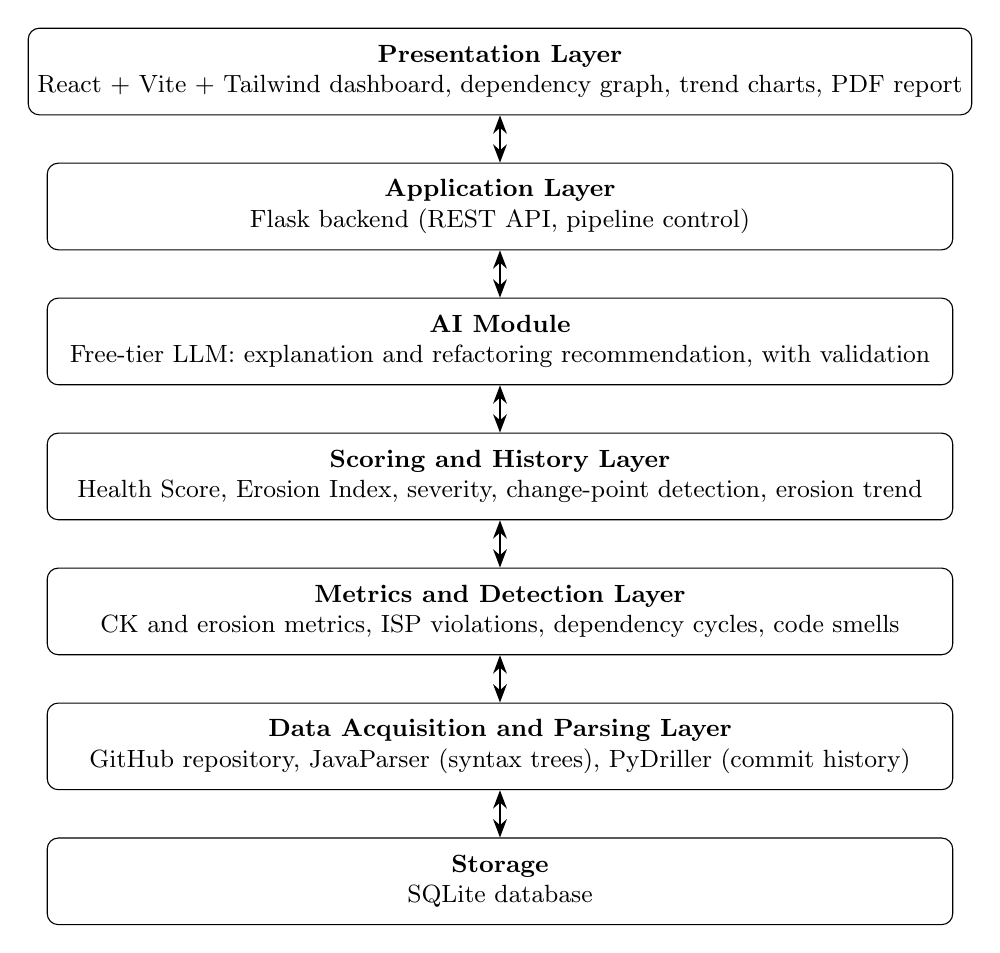
\begin{tikzpicture}[
  node distance=6mm,
  box/.style={
    draw,
    rounded corners,
    minimum width=11.5cm,
    minimum height=1.1cm,
    align=center,
    font=\small
  },
  arr/.style={{Stealth}-{Stealth},thick}
]
\node[box] (ui) {
  \textbf{Presentation Layer}\\
  React + Vite + Tailwind dashboard, dependency graph, trend charts, PDF report
};

\node[box,below=of ui] (api) {
  \textbf{Application Layer}\\
  Flask backend (REST API, pipeline control)
};

\node[box,below=of api] (ai) {
  \textbf{AI Module}\\
  Free-tier LLM: explanation and refactoring recommendation, with validation
};

\node[box,below=of ai] (score) {
  \textbf{Scoring and History Layer}\\
  Health Score, Erosion Index, severity, change-point detection, erosion trend
};

\node[box,below=of score] (det) {
  \textbf{Metrics and Detection Layer}\\
  CK and erosion metrics, ISP violations, dependency cycles, code smells
};

\node[box,below=of det] (parse) {
  \textbf{Data Acquisition and Parsing Layer}\\
  GitHub repository, JavaParser (syntax trees), PyDriller (commit history)
};

\node[box,below=of parse] (db) {
  \textbf{Storage}\\
  SQLite database
};

\draw[arr] (ui) -- (api);
\draw[arr] (api) -- (ai);
\draw[arr] (ai) -- (score);
\draw[arr] (score) -- (det);
\draw[arr] (det) -- (parse);
\draw[arr] (parse) -- (db);

\end{tikzpicture}
\caption{Basic architecture of InterfaceGuard}
\label{fig:arch}
\end{figure}

\clearpage

% ============================================================
% CHAPTER 2: SYSTEM STUDY AND ANALYSIS
% ============================================================
\section{SYSTEM STUDY AND ANALYSIS}

\begin{spacing}{1.5}
\justifying
This chapter studies the problem that InterfaceGuard addresses. It examines
the limitations of the tools developers use today, states the problem
formally, assesses whether the proposed solution is feasible, presents the
project plan, and lists the requirements the system must satisfy.
\end{spacing}

% ------------------------------------------------------------
\subsection{Drawbacks of the Existing System}

\begin{spacing}{1.5}
\justifying
Developers currently rely on free static analysis tools that compute
object-oriented metrics and detect code smells, and on commercial
code-quality platforms that offer more but require paid licences. For
the specific problem of interface erosion, these tools have the following
drawbacks:

\begin{itemize}[leftmargin=*,itemsep=3pt]
  \item \textbf{Single-snapshot analysis:} Metrics and smells are reported
        for one version of the code. The tools do not track how the design
        quality of an interface changes across a project's commit history.

  \item \textbf{No onset detection:} They cannot show \emph{when} an
        interface began to degrade, or which commit and author introduced
        the change.

  \item \textbf{No interface-level view:} Results are reported mainly per
        class or per file. Interface-specific symptoms, such as method-count
        growth, interface churn, breaking changes and low interface cohesion,
        are not measured.

  \item \textbf{No trend information:} A developer cannot tell whether
        an interface is stable, slowly worsening or degrading at an
        accelerating rate.

  \item \textbf{Limited ISP detection:} Violations of the Interface
        Segregation Principle, such as implementing classes with empty,
        no-operation or exception-throwing method bodies, are not reliably
        flagged.

  \item \textbf{Raw output only:} Metrics are presented as numbers and
        warnings without a plain-language explanation or a concrete
        refactoring suggestion, which is a particular difficulty for
        students and junior developers.

  \item \textbf{Cost barrier:} Commercial platforms that offer richer
        reporting have licensing costs that small teams and student
        projects often cannot afford.
\end{itemize}
\end{spacing}

% ------------------------------------------------------------
\subsection{Problem Statement}

\begin{spacing}{1.5}
\justifying
As object-oriented software evolves through repeated modifications,
interfaces and class relationships gradually deteriorate. Interfaces
accumulate unrelated responsibilities, a problem known as
\emph{interface erosion}, which appears as bloated interfaces, violations
of the Interface Segregation Principle (ISP), cyclic dependencies, rising
coupling, and implementing classes forced to write empty or unused method
bodies. This increases technical debt and maintenance cost.

There is a need for a free tool that detects interface erosion, shows how
it develops over time, shows which interfaces are getting worse, and
explains clearly to the developer what to do about it. InterfaceGuard is
developed to meet this need.
\end{spacing}

% ------------------------------------------------------------
\subsection{Feasibility Study}

\begin{spacing}{1.5}
\justifying
A feasibility study was carried out to confirm that the project can be
completed within the available time, budget and resources.
\end{spacing}

\subsubsection{Technical Feasibility}

\begin{spacing}{1.5}
\justifying
The project is technically feasible because every major function is
supported by a mature, well-documented library, so no parser, Git-mining
logic, graph algorithm or change-point algorithm has to be written from
scratch (Table~\ref{tab:techfeas}). React with Vite and Tailwind CSS gives
a fast frontend workflow, and Recharts and React Flow provide ready-made
charting and graph components. The system runs on a standard laptop with
8~GB RAM and needs no GPU.
\end{spacing}

% ---------- TECHNOLOGY FEASIBILITY TABLE ----------
\begin{table}[htbp]
\centering
\label{tab:techfeas}
\renewcommand{\arraystretch}{1.5}
\setlength{\tabcolsep}{6pt}

\begin{tabular}{|L{1.9in}|L{3.45in}|}
\hline
\textbf{Function} & \textbf{Supporting Technology} \\
\hline
Java Parsing and Type Resolution
    & JavaParser, JavaSymbolSolver \\
\hline
Git History Mining
    & PyDriller \\
\hline
Dependency Graph and Cycle Detection
    & NetworkX \\
\hline
Change-Point Detection
    & ruptures, SciPy \\
\hline
Explanations and Refactoring Recommendations
    & Free-tier LLM API (e.g., Google Gemini) \\
\hline
Backend and Data Storage
    & Python Flask, SQLite \\
\hline
Dashboard and Visualizations
    & React, Vite, Tailwind CSS, Recharts, React Flow / D3 \\
\hline
PDF Report Generation
    & WeasyPrint \\
\hline
\end{tabular}
\end{table}

% ------------------------------------------------------------
\subsubsection{Economic Feasibility}

\begin{spacing}{1.5}
\justifying
All software used is free and open-source. The LLM component relies on
free-tier API credits, which are sufficient for the test repositories,
and responses are cached to stay within rate limits. No paid hosting,
database or cloud service is needed, because the whole prototype runs
locally. The cost of development is therefore limited to the developer's
own laptop and time.
\end{spacing}

% ------------------------------------------------------------
\subsubsection{Operational Feasibility}

\begin{spacing}{1.5}
\justifying
The system is operated entirely from a web dashboard: the user pastes
a public GitHub URL and reads the results. No installation of analysis
tools on the user's side and no knowledge of the underlying metrics is
required, because findings are accompanied by plain-language explanations.
The tool fits naturally into the review habits of students and small teams.
\end{spacing}

% ------------------------------------------------------------
\subsubsection{Schedule Feasibility}

\begin{spacing}{1.5}
\justifying
The scope can be completed in about three months. The work is divided
into six two-week sprints (Section~\ref{sec:planning}), and each sprint
depends only on libraries that are already available.
\end{spacing}

% ------------------------------------------------------------

\subsubsection{Risks and Mitigation}

\begin{table}[htbp]
\centering
\label{tab:risks}
\renewcommand{\arraystretch}{1.5}
\setlength{\tabcolsep}{8pt}

\begin{tabular}{|L{2.0in}|L{3.35in}|}
\hline
\textbf{Risk} & \textbf{Mitigation} \\
\hline
Free-tier LLM rate limits
& Cache responses and send requests only for flagged interfaces. \\
\hline
Incorrect or invented LLM suggestions
& Verify that every method named in a suggestion exists in the source code and label the output as AI-generated. \\
\hline
Large repositories are slow to analyse
& Analyse selected commits rather than every commit and use smaller test repositories during development. \\
\hline
Repositories with little history
& Select test repositories with sufficient and meaningful commit history for historical analysis. \\
\hline
\end{tabular}
\end{table}


% ------------------------------------------------------------
\subsection{Project Planning}
\label{sec:planning}

\begin{spacing}{1.5}
\justifying
The project is planned over three months and organised as six two-week
sprints, following an incremental approach in which each sprint ends with
a working, demonstrable part of the system. Table~\ref{tab:plan} gives
the plan.
\end{spacing}

\begin{table}[htbp]
\centering
\label{tab:plan}
\renewcommand{\arraystretch}{1.5}
\setlength{\tabcolsep}{8pt}

\begin{tabular}{|L{0.9in}|L{0.9in}|L{3.55in}|}
\hline
\textbf{Month} & \textbf{Sprint} & \textbf{Activities} \\
\hline

1 & 1--2
& Repository import, JavaParser setup, interface extraction, CK and
interface erosion metrics, ISP violation detection, dependency and
cycle detection. \\
\hline

2 & 3--4
& Code-smell detection, Health Score, Erosion Index and severity
classes, Git history tracking, change-point detection, erosion
trend analysis, and labelling of the evaluation sample. \\
\hline

3 & 5--6
& LLM explanations and refactoring recommendations, React/Vite/Tailwind
dashboard with dependency graph and trend charts, PDF reporting,
evaluation on sample repositories, and documentation. \\
\hline

\end{tabular}
\end{table}

% ------------------------------------------------------------
\subsection{Requirement Specification}

\subsubsection{Functional Requirements}

\begin{enumerate}[leftmargin=*,itemsep=2pt,label=FR\arabic*.]
  \item The system shall accept a public GitHub repository URL and clone it.

  \item The system shall parse Java source files and extract interfaces,
        their methods and their implementing classes.

  \item The system shall analyse the Git commit history and examine the
        code at selected commits.

  \item The system shall compute the CK metrics (CBO, LCOM, RFC, WMC, DIT,
        NOC) and the interface erosion metrics (method-count growth,
        interface churn, breaking change count, interface cohesion).

  \item The system shall detect ISP violations, dependency cycles and code
        smells (God Class, Large Class, Long Method, Feature Envy,
        Refused Bequest, Fat Interface).

  \item The system shall compute an Interface Health Score (0--100) for
        each interface, a project-level Erosion Index, and a severity
        class (Low, Medium, High, Critical).

  \item The system shall detect the change point at which an interface
        begins to erode and classify its trend as Stable, Rising or
        Accelerating.

  \item The system shall generate a plain-language explanation and a
        refactoring recommendation for each flagged interface using an
        LLM, verify that the methods it names exist, and label it as
        AI-generated.

  \item The system shall present results on an interactive dashboard
        with a project overview, a per-interface detail view, a dependency
        graph and trend charts.

  \item The system shall export the findings as a downloadable PDF report.
\end{enumerate}

% ------------------------------------------------------------
\subsubsection{Non-Functional Requirements}

\begin{itemize}[leftmargin=*,itemsep=2pt]
  \item \textbf{Cost:} only free and open-source software is used.

  \item \textbf{Performance:} analysis of the small test repositories
        completes on a laptop without a GPU; LLM responses are cached.

  \item \textbf{Usability:} a user can start an analysis with a single
        URL and interpret the results without prior knowledge of the metrics.

  \item \textbf{Reliability:} the system reports a clear error for invalid
        or inaccessible repositories and does not crash on unparsable files.

  \item \textbf{Trustworthiness:} AI-generated content is clearly labelled
        and checked against the actual code.

  \item \textbf{Portability:} the prototype runs locally on a standard
        personal computer.
\end{itemize}

% ------------------------------------------------------------
\subsubsection{Hardware Requirements}

\begin{table}[H]
\centering
\label{tab:hw}
\renewcommand{\arraystretch}{1.4}
\setlength{\tabcolsep}{8pt}

\begin{tabular}{|L{1.6in}|L{3.75in}|}
\hline
\textbf{Component} & \textbf{Requirement} \\
\hline
Processor & Intel Core i5 or equivalent processor. \\
\hline
RAM & Minimum 8~GB. \\
\hline
Storage & At least 10~GB of free storage for cloned repositories and project files. \\
\hline
GPU & Not required. \\
\hline
Network & Internet connection for GitHub repository access and LLM API integration. \\
\hline
\end{tabular}
\end{table}

% ------------------------------------------------------------
\subsubsection{Software Requirements}

\begin{table}[htbp]
\centering
\label{tab:sw}
\renewcommand{\arraystretch}{1.4}
\setlength{\tabcolsep}{8pt}

\begin{tabular}{|L{1.6in}|L{3.75in}|}
\hline
\textbf{Item} & \textbf{Details} \\
\hline
Operating System & Windows 11. \\
\hline
Programming Languages & Python for analysis and backend development, Java for the analysed source code, and JavaScript for frontend development. \\
\hline
Backend & Flask for the backend API and SQLite for database storage. \\
\hline
Analysis Libraries & JavaParser, JavaSymbolSolver, PyDriller, NetworkX, ruptures, and SciPy. \\
\hline
Frontend & React, Vite, Tailwind CSS, Recharts, and React Flow or D3 for visualisations. \\
\hline
Reporting & WeasyPrint for generating PDF reports. \\
\hline
AI Integration & A compatible free-tier LLM API, such as Google Gemini, for explanations and refactoring recommendations. \\
\hline
Development Tools & Git, Node.js, Visual Studio Code or another suitable IDE, and a web browser. \\
\hline
\end{tabular}
\end{table}

\clearpage

% ============================================================
% CHAPTER 3: SYSTEM WORK FLOW
% ============================================================
\section{SYSTEM WORK FLOW}

\begin{spacing}{1.5}
\justifying
This chapter describes how InterfaceGuard was designed and how it behaves.
It explains the design methodology, presents the UML diagrams that model
the structure and behaviour of the system, and describes the use cases
through which a user interacts with it.
\end{spacing}

% ------------------------------------------------------------
\subsection{Design Methodology}

\begin{spacing}{1.5}
\justifying
InterfaceGuard was designed using an \emph{object-oriented analysis and
design} approach modelled with the Unified Modeling Language (UML), and it
was built using an \emph{incremental, sprint-based} development process.
\end{spacing}

% ------------------------------------------------------------
\subsubsection{Development Process}

\begin{spacing}{1.5}
\justifying
The project is divided into six two-week sprints (Section~\ref{sec:planning}).
Each sprint adds one working part of the pipeline, for example parsing, then
metrics, then scoring, and ends with a demonstrable result. Because the
output of each stage is the input of the next, the parts can be built and
tested one after the other, and problems are found early rather than at final
integration.
\end{spacing}

% ------------------------------------------------------------
\subsubsection{Pipeline Architecture}

\begin{spacing}{1.5}
\justifying
Within the layered architecture described in Section~1.6, the analysis
itself follows a \emph{pipeline} style. Data flows in one direction through
independent stages, and each stage hides its internals behind a small,
clearly defined interface. The stages, with their inputs and outputs, are
listed in the table below.
\end{spacing}

\begin{table}[H]
\centering
\renewcommand{\arraystretch}{1.5}
\setlength{\tabcolsep}{6pt}

\begin{tabular}{|L{1.4in}|L{1.9in}|L{2.05in}|}
\hline
\textbf{Stage} & \textbf{Input} & \textbf{Output} \\
\hline
Acquisition & GitHub URL & Source files and commit list \\
\hline
Parsing & Source files & Interfaces, methods and implementing classes \\
\hline
Metrics & Interface snapshots & CK and interface erosion metrics \\
\hline
Detection & Snapshots and metrics & ISP violations, dependency cycles, code smells \\
\hline
Scoring & Indicators & Health Score, Erosion Index, severity class \\
\hline
History analysis & Health Score series & Change point, onset commit, erosion trend \\
\hline
AI explanation & Flagged interface details & Explanation and refactoring recommendation \\
\hline
Presentation & Stored results & Dashboard views and PDF report \\
\hline
\end{tabular}
\end{table}

% ------------------------------------------------------------
\subsubsection{Design Principles Applied}

\begin{spacing}{1.5}
\justifying
The principles listed in Section~1.5 apply throughout the work flow. Three of
them shape it directly.

\begin{itemize}[leftmargin=*,itemsep=2pt]
  \item \textbf{Small, focused interfaces:} each module exposes only the
        operations its clients need, in keeping with the Interface
        Segregation Principle that the tool itself is built to check.

  \item \textbf{Rules first, AI second:} all measurements and detections
        are computed by deterministic, rule-based code. The LLM is used only
        to explain findings, and its output is validated against the actual
        code.

  \item \textbf{Reproducibility:} results and LLM responses are cached in
        SQLite, so the same analysis gives the same output and free-tier
        rate limits are respected.
\end{itemize}
\end{spacing}

% ------------------------------------------------------------
\subsection{UML Diagrams}

\begin{spacing}{1.5}
\justifying
Four UML diagrams model InterfaceGuard: a class diagram for its static
structure, a sequence diagram for the order of interactions during an
analysis, an activity diagram for the overall work flow, and, in
Section~\ref{sec:usecase}, a use case diagram for the user's view of the
system.
\end{spacing}

% ------------------------------------------------------------
\subsubsection{Class Diagram}

\begin{spacing}{1.5}
\justifying
Figure~\ref{fig:class} shows the main classes. The entity classes
\textit{Repository}, \textit{Commit} and \textit{Interface\-Snapshot} hold the
data; the remaining classes are the processing modules that read and enrich
\textit{Interface\-Snapshot} objects.
\end{spacing}

\begin{figure}[htbp]
\centering
\resizebox{\linewidth}{!}{%
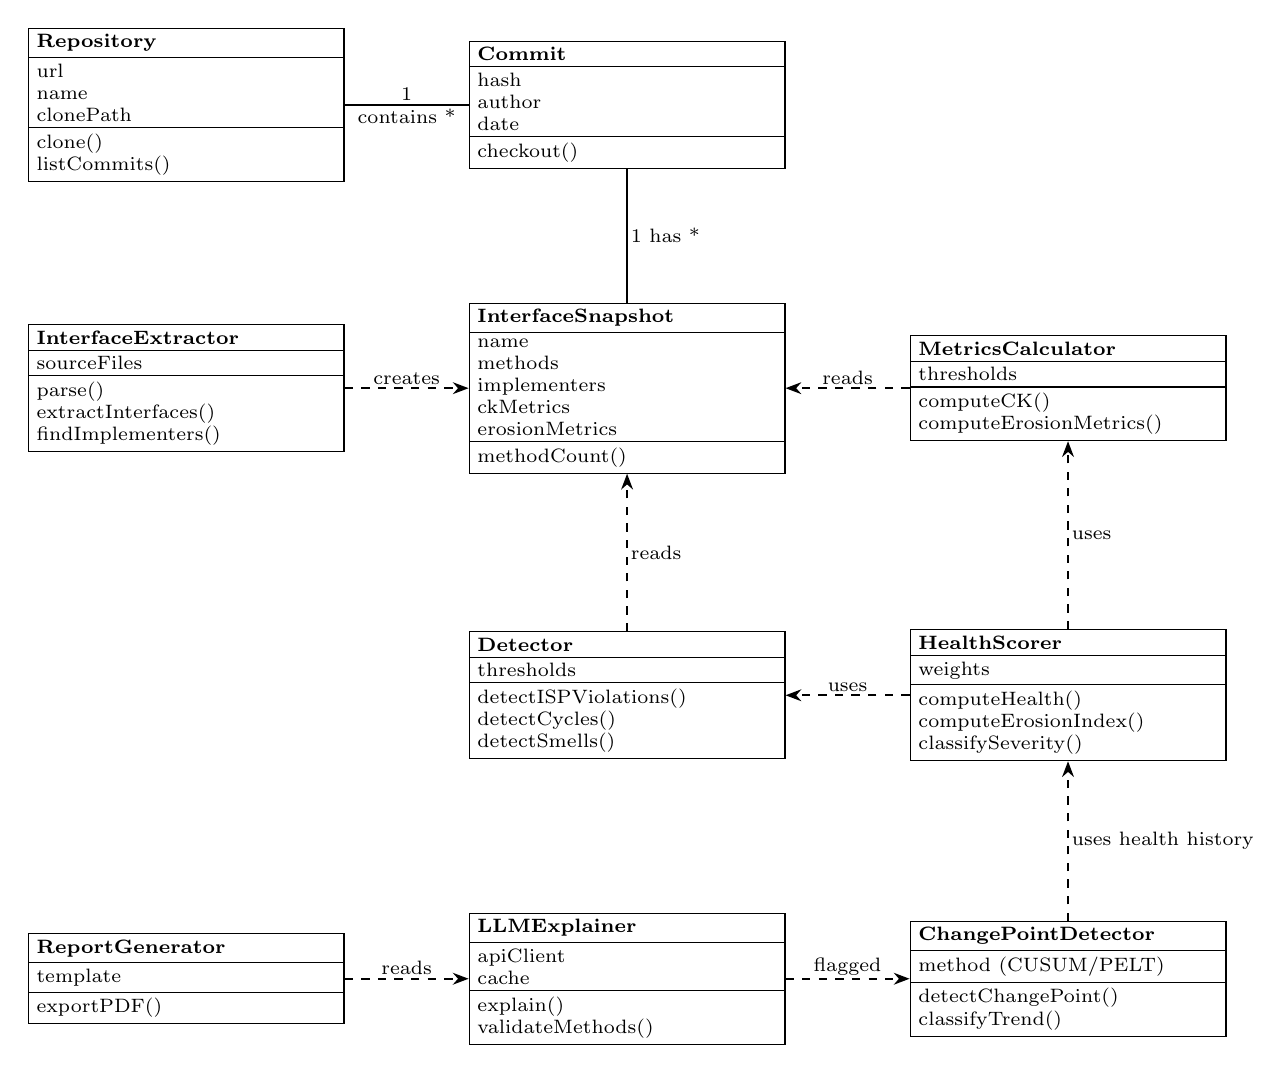
\begin{tikzpicture}[
  scale=1, transform shape,
  cls/.style={rectangle split, rectangle split parts=3, draw, fill=white,
              font=\scriptsize, text width=3.8cm, align=left,
              inner xsep=3pt, inner ysep=2pt},
  hdr/.style={font=\scriptsize\bfseries},
  assoc/.style={thick},
  dep/.style={thick,dashed,-{Stealth[length=2mm]}},
  lab/.style={font=\scriptsize,fill=white,inner sep=1pt}
]
% ---- Row 1 ----
\node[cls] (repo) at (0,0)
 {\centering\textbf{Repository}
  \nodepart{second}url\\name\\clonePath
  \nodepart{third}clone()\\listCommits()};
\node[cls] (commit) at (5.6,0)
 {\centering\textbf{Commit}
  \nodepart{second}hash\\author\\date
  \nodepart{third}checkout()};
% ---- Row 2 ----
\node[cls] (ext) at (0,-3.6)
 {\centering\textbf{InterfaceExtractor}
  \nodepart{second}sourceFiles
  \nodepart{third}parse()\\extractInterfaces()\\findImplementers()};
\node[cls] (snap) at (5.6,-3.6)
 {\centering\textbf{InterfaceSnapshot}
  \nodepart{second}name\\methods\\implementers\\ckMetrics\\erosionMetrics
  \nodepart{third}methodCount()};
\node[cls] (met) at (11.2,-3.6)
 {\centering\textbf{MetricsCalculator}
  \nodepart{second}thresholds
  \nodepart{third}computeCK()\\computeErosionMetrics()};
% ---- Row 3 ----
\node[cls] (det) at (5.6,-7.5)
 {\centering\textbf{Detector}
  \nodepart{second}thresholds
  \nodepart{third}detectISPViolations()\\detectCycles()\\detectSmells()};
\node[cls] (score) at (11.2,-7.5)
 {\centering\textbf{HealthScorer}
  \nodepart{second}weights
  \nodepart{third}computeHealth()\\computeErosionIndex()\\classifySeverity()};
% ---- Row 4 ----
\node[cls] (cp) at (11.2,-11.1)
 {\centering\textbf{ChangePointDetector}
  \nodepart{second}method (CUSUM/PELT)
  \nodepart{third}detectChangePoint()\\classifyTrend()};
\node[cls] (llm) at (5.6,-11.1)
 {\centering\textbf{LLMExplainer}
  \nodepart{second}apiClient\\cache
  \nodepart{third}explain()\\validateMethods()};
\node[cls] (rep) at (0,-11.1)
 {\centering\textbf{ReportGenerator}
  \nodepart{second}template
  \nodepart{third}exportPDF()};

% ---- Relationships ----
\draw[assoc] (repo.east) -- node[lab,above]{1} node[lab,below]{contains *} (commit.west);
\draw[assoc] (commit.south) -- node[lab,right]{1 has *} (snap.north);
\draw[dep] (ext.east) -- node[lab,above]{creates} (snap.west);
\draw[dep] (met.west) -- node[lab,above]{reads} (snap.east);
\draw[dep] (det.north) -- node[lab,right]{reads} (snap.south);
\draw[dep] (score.north) -- node[lab,right]{uses} (met.south);
\draw[dep] (score.west) -- node[lab,above]{uses} (det.east);
\draw[dep] (cp.north) -- node[lab,right]{uses health history} (score.south);
\draw[dep] (llm.east) -- node[lab,above]{flagged} (cp.west);
\draw[dep] (rep.east) -- node[lab,above]{reads} (llm.west);
\end{tikzpicture}}
\caption{Class diagram of InterfaceGuard}
\label{fig:class}
\end{figure}

% ------------------------------------------------------------
\subsubsection{Sequence Diagram}

\begin{spacing}{1.5}
\justifying
Figure~\ref{fig:seq} shows the interactions during one analysis. The user
submits a URL on the dashboard; the Flask API starts the analysis; the
analyzer clones the repository from GitHub, computes metrics and scores, and
asks the LLM to explain flagged interfaces; the results are stored in SQLite
and finally read back by the dashboard.
\end{spacing}

\begin{figure}[htbp]
\centering
\resizebox{\linewidth}{!}{%
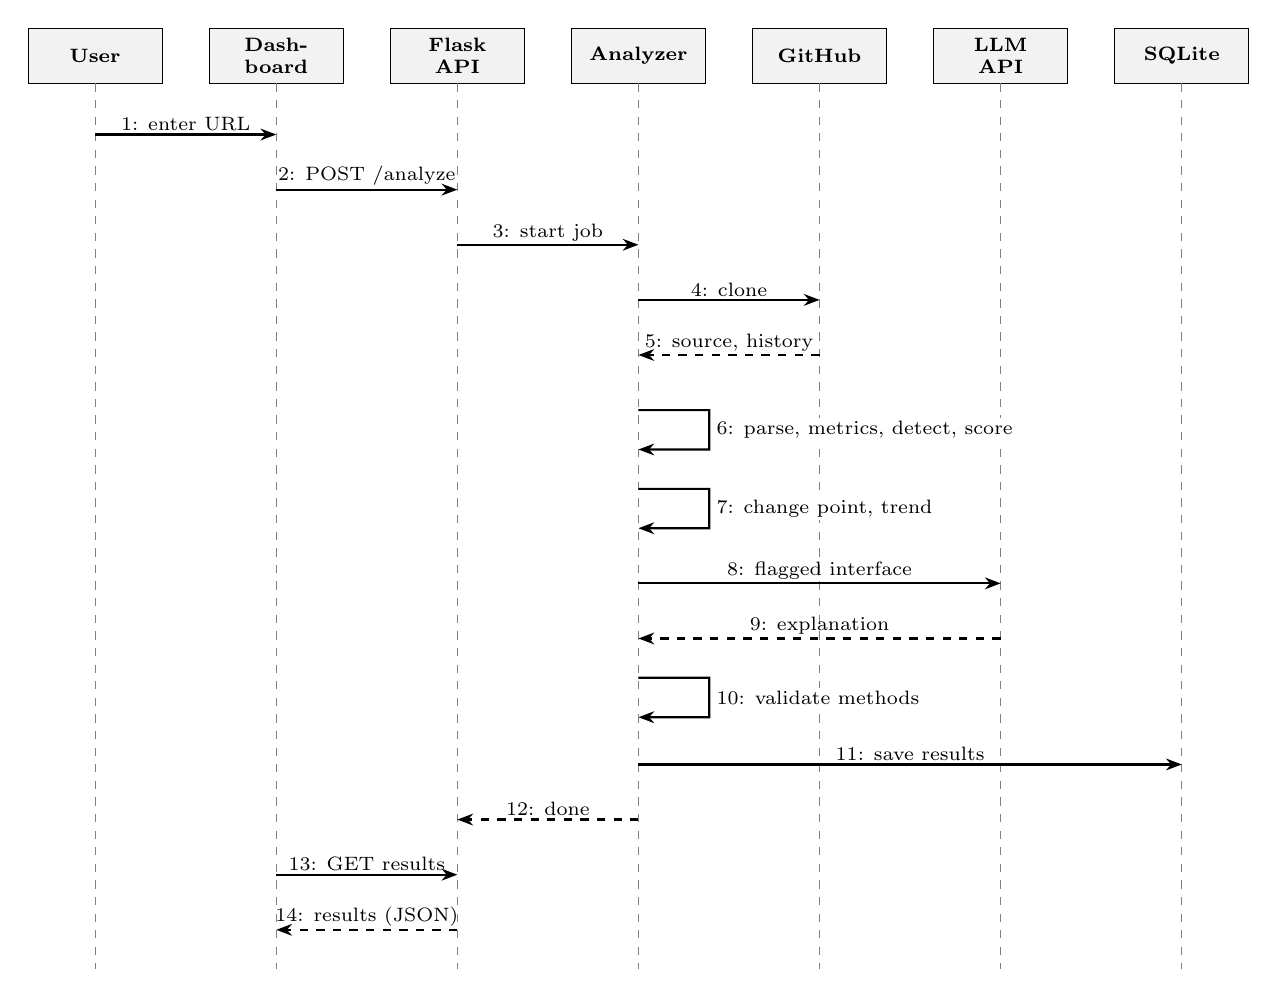
\begin{tikzpicture}[
  x=1cm,y=1cm,
  life/.style={font=\scriptsize\bfseries,draw,fill=gray!10,minimum width=1.7cm,
               minimum height=0.7cm,align=center},
  ll/.style={dashed,gray},
  msg/.style={-{Stealth[length=2mm]},thick},
  ret/.style={-{Stealth[length=2mm]},thick,dashed},
  ml/.style={font=\scriptsize,above,align=center,inner sep=1pt}
]
\def\top{0}
\def\bot{-11.6}
% x positions
\def\xu{0}   \def\xd{2.3}  \def\xa{4.6}  \def\xz{6.9}
\def\xg{9.2} \def\xl{11.5} \def\xs{13.8}
\node[life] (u) at (\xu,\top) {User};
\node[life] (d) at (\xd,\top) {Dash-\\board};
\node[life] (a) at (\xa,\top) {Flask\\API};
\node[life] (z) at (\xz,\top) {Analyzer};
\node[life] (g) at (\xg,\top) {GitHub};
\node[life] (l) at (\xl,\top) {LLM\\API};
\node[life] (s) at (\xs,\top) {SQLite};
\foreach \x in {\xu,\xd,\xa,\xz,\xg,\xl,\xs}
  \draw[ll] (\x,-0.35) -- (\x,\bot);

\draw[msg] (\xu,-1.0) -- node[ml]{1: enter URL} (\xd,-1.0);
\draw[msg] (\xd,-1.7) -- node[ml]{2: POST /analyze} (\xa,-1.7);
\draw[msg] (\xa,-2.4) -- node[ml]{3: start job} (\xz,-2.4);
\draw[msg] (\xz,-3.1) -- node[ml]{4: clone} (\xg,-3.1);
\draw[ret] (\xg,-3.8) -- node[ml]{5: source, history} (\xz,-3.8);
% self messages on Analyzer
\draw[msg] (\xz,-4.5) -- ++(0.9,0) -- ++(0,-0.5) -- node[ml,right,xshift=1pt,above=0pt]{} (\xz,-5.0);
\node[font=\scriptsize,anchor=west,fill=white,inner sep=1pt] at (\xz+0.95,-4.75) {6: parse, metrics, detect, score};
\draw[msg] (\xz,-5.5) -- ++(0.9,0) -- ++(0,-0.5) -- (\xz,-6.0);
\node[font=\scriptsize,anchor=west,fill=white,inner sep=1pt] at (\xz+0.95,-5.75) {7: change point, trend};
\draw[msg] (\xz,-6.7) -- node[ml]{8: flagged interface} (\xl,-6.7);
\draw[ret] (\xl,-7.4) -- node[ml]{9: explanation} (\xz,-7.4);
\draw[msg] (\xz,-7.9) -- ++(0.9,0) -- ++(0,-0.5) -- (\xz,-8.4);
\node[font=\scriptsize,anchor=west,fill=white,inner sep=1pt] at (\xz+0.95,-8.15) {10: validate methods};
\draw[msg] (\xz,-9.0) -- node[ml]{11: save results} (\xs,-9.0);
\draw[ret] (\xz,-9.7) -- node[ml]{12: done} (\xa,-9.7);
\draw[msg] (\xd,-10.4) -- node[ml]{13: GET results} (\xa,-10.4);
\draw[ret] (\xa,-11.1) -- node[ml]{14: results (JSON)} (\xd,-11.1);
\end{tikzpicture}}
\caption{Sequence diagram of one repository analysis}
\label{fig:seq}
\end{figure}

% ------------------------------------------------------------
\subsubsection{Activity Diagram}

\begin{spacing}{1.5}
\justifying
Figure~\ref{fig:activity} shows the overall work flow of the system,
including the loop that repeats the analysis for every selected commit and
the decision that sends only flagged interfaces to the LLM.
\end{spacing}

\begin{figure}[htbp]
\centering
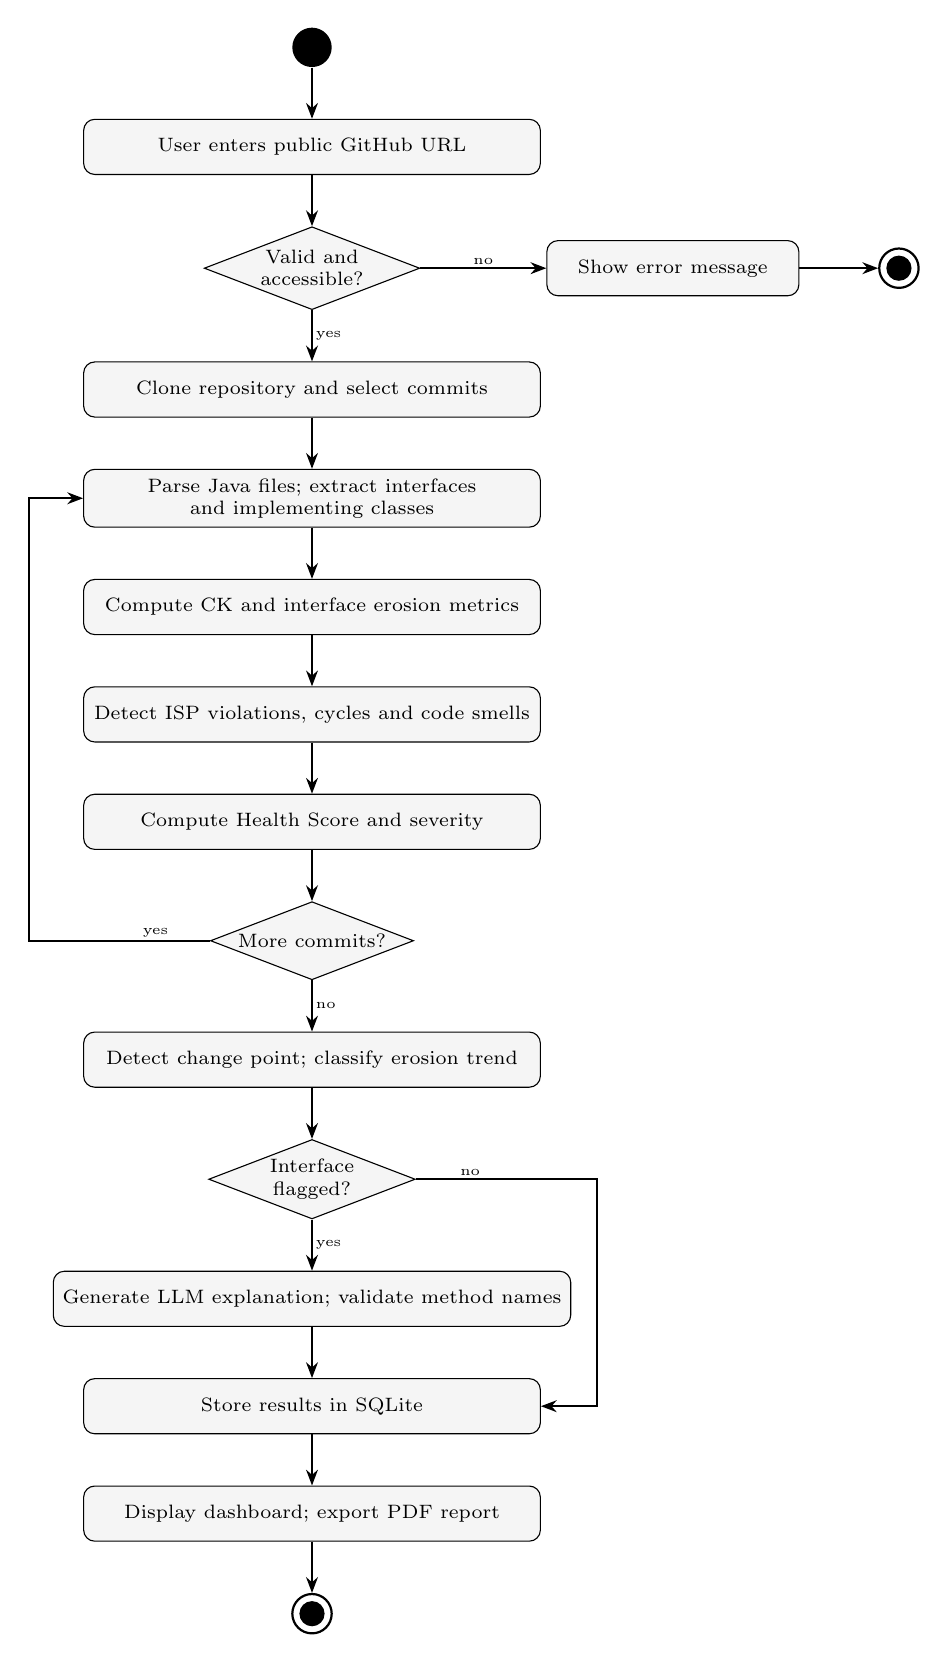
\begin{tikzpicture}[
  node distance=6.5mm,
  act/.style={draw,rounded corners=4pt,align=center,font=\scriptsize,
              minimum height=7mm,minimum width=5.8cm,fill=gray!8},
  dec/.style={draw,diamond,aspect=2.6,align=center,font=\scriptsize,
              inner sep=1pt,fill=gray!8},
  st/.style={circle,fill=black,minimum size=5mm},
  en/.style={circle,draw,thick,minimum size=5mm,
             path picture={\fill (path picture bounding box.center) circle (1.6mm);}},
  arr/.style={-{Stealth[length=2mm]},thick},
  lab/.style={font=\tiny,inner sep=1pt}
]
\node[st] (s) {};
\node[act,below=of s] (a1) {User enters public GitHub URL};
\node[dec,below=of a1] (d1) {Valid and\\accessible?};
\node[act,below=of d1] (a2) {Clone repository and select commits};
\node[act,below=of a2] (a3) {Parse Java files; extract interfaces\\and implementing classes};
\node[act,below=of a3] (a4) {Compute CK and interface erosion metrics};
\node[act,below=of a4] (a5) {Detect ISP violations, cycles and code smells};
\node[act,below=of a5] (a6) {Compute Health Score and severity};
\node[dec,below=of a6] (d2) {More commits?};
\node[act,below=of d2] (a7) {Detect change point; classify erosion trend};
\node[dec,below=of a7] (d3) {Interface\\flagged?};
\node[act,below=of d3] (a8) {Generate LLM explanation; validate method names};
\node[act,below=of a8] (a9) {Store results in SQLite};
\node[act,below=of a9] (a10) {Display dashboard; export PDF report};
\node[en,below=of a10] (e) {};
% error branch
\node[act,right=1.6cm of d1,minimum width=3.2cm] (err) {Show error message};
\node[en,right=1cm of err] (e2) {};

\draw[arr] (s)--(a1); \draw[arr] (a1)--(d1);
\draw[arr] (d1)--node[lab,right]{yes}(a2);
\draw[arr] (d1)--node[lab,above]{no}(err);
\draw[arr] (err)--(e2);
\draw[arr] (a2)--(a3); \draw[arr] (a3)--(a4); \draw[arr] (a4)--(a5);
\draw[arr] (a5)--(a6); \draw[arr] (a6)--(d2);
\draw[arr] (d2)--node[lab,right]{no}(a7);
% loop back
\draw[arr] (d2.west) -- node[lab,above,pos=0.3]{yes} ++(-2.3,0) |- (a3.west);
\draw[arr] (a7)--(d3);
\draw[arr] (d3)--node[lab,right]{yes}(a8);
\draw[arr] (d3.east) -- node[lab,above,pos=0.3]{no} ++(2.3,0) |- (a9.east);
\draw[arr] (a8)--(a9); \draw[arr] (a9)--(a10); \draw[arr] (a10)--(e);
\end{tikzpicture}
\caption{Activity diagram of the analysis work flow}
\label{fig:activity}
\end{figure}

% ------------------------------------------------------------
\subsection{Use Case Design}
\label{sec:usecase}

% ------------------------------------------------------------
\subsubsection{Actors}

\begin{spacing}{1.5}
\justifying
\begin{itemize}[leftmargin=*,itemsep=2pt]
  \item \textbf{Developer / Student (primary actor):} supplies a repository,
        reviews the findings and downloads the report.

  \item \textbf{GitHub (secondary actor):} provides the repository source
        and its commit history.

  \item \textbf{LLM API (secondary actor):} provides the explanation and
        refactoring text for flagged interfaces.
\end{itemize}
\end{spacing}

% ------------------------------------------------------------
\subsubsection{Use Case Diagram}

\begin{spacing}{1.5}
\justifying
Figure~\ref{fig:usecase} shows the use cases. \emph{Run Analysis} is
triggered when a repository is submitted and includes the parsing, scoring,
change-point and AI-explanation steps.
\end{spacing}

\begin{figure}[htbp]
\centering
\resizebox{\linewidth}{!}{%
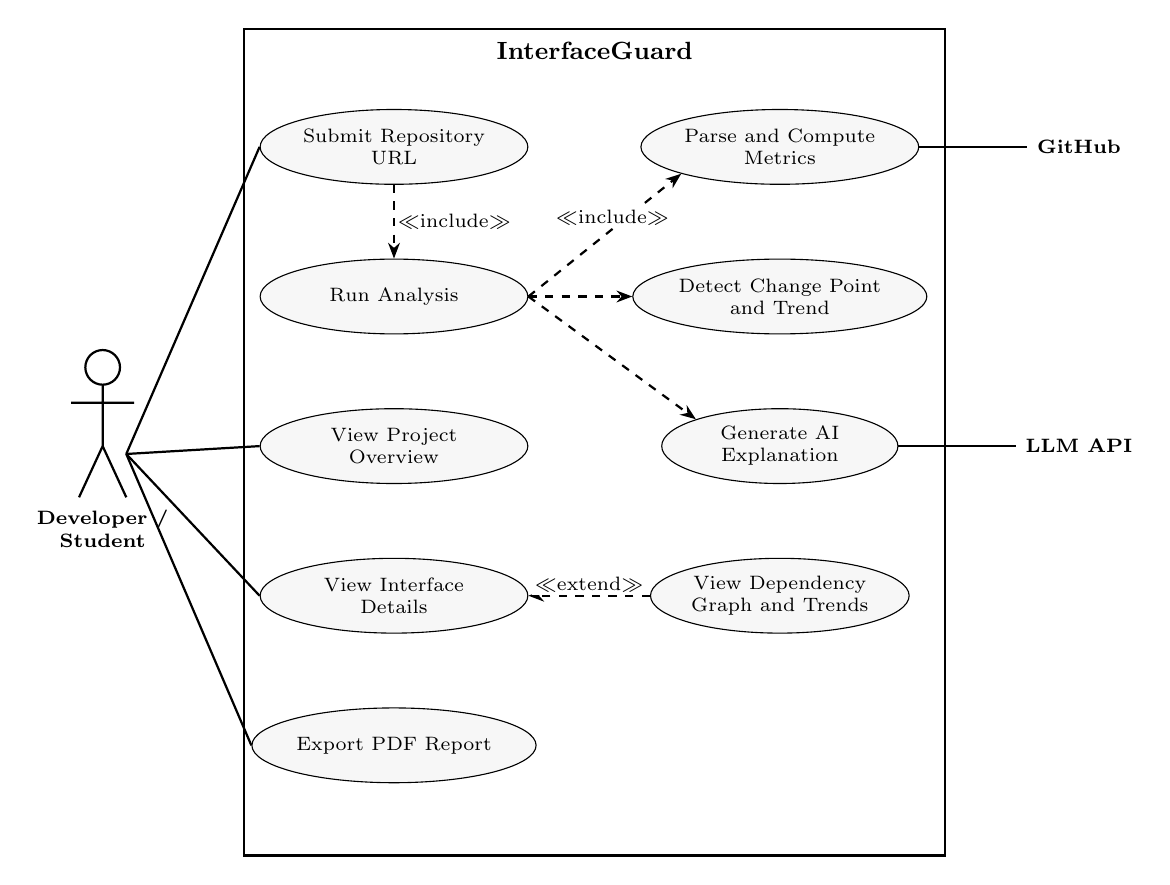
\begin{tikzpicture}[
  actor/.style={align=center,font=\scriptsize\bfseries},
  uc/.style={draw,ellipse,align=center,font=\scriptsize,minimum width=3.4cm,
             minimum height=0.95cm,fill=gray!6,inner sep=1pt},
  assoc/.style={thick},
  inc/.style={dashed,-{Stealth[length=2mm]},thick},
  lab/.style={font=\scriptsize,fill=white,inner sep=1pt}
]
% system boundary
\draw[thick] (2.4,-9.3) rectangle (11.3,1.2);
\node[font=\small\bfseries,anchor=north] at (6.85,1.15) {InterfaceGuard};

% stick figure for Developer
\begin{scope}[shift={(0.6,-4)}]
  \draw[thick] (0,0.9) circle (0.22);
  \draw[thick] (0,0.68)--(0,-0.1) (-0.4,0.45)--(0.4,0.45)
        (0,-0.1)--(-0.3,-0.75) (0,-0.1)--(0.3,-0.75);
  \node[actor] at (0,-1.15) {Developer /\\Student};
\end{scope}

% use cases
\node[uc] (u1) at (4.3,-0.3) {Submit Repository\\URL};
\node[uc] (u2) at (4.3,-2.2) {Run Analysis};
\node[uc] (u3) at (4.3,-4.1) {View Project\\Overview};
\node[uc] (u4) at (4.3,-6.0) {View Interface\\Details};
\node[uc] (u5) at (4.3,-7.9) {Export PDF Report};

\node[uc,minimum width=3.0cm] (i1) at (9.2,-0.3) {Parse and Compute\\Metrics};
\node[uc,minimum width=3.0cm] (i2) at (9.2,-2.2) {Detect Change Point\\and Trend};
\node[uc,minimum width=3.0cm] (i3) at (9.2,-4.1) {Generate AI\\Explanation};
\node[uc,minimum width=3.0cm] (i4) at (9.2,-6.0) {View Dependency\\Graph and Trends};

% actor to use cases
\foreach \u in {u1,u3,u4,u5} \draw[assoc] (0.9,-4.2) -- (\u.west);
% submit includes run analysis
\draw[inc] (u1) -- node[lab,right]{$\ll$include$\gg$} (u2);
% run analysis includes
\draw[inc] (u2.east) -- node[lab,above,pos=0.55]{$\ll$include$\gg$} (i1.south west);
\draw[inc] (u2.east) -- (i2.west);
\draw[inc] (u2.east) -- (i3.north west);
% detail view extends/includes graph view
\draw[inc] (i4.west) -- node[lab,above]{$\ll$extend$\gg$} (u4.east);

% external actors (right)
\node[actor] (gh) at (13.0,-0.3) {GitHub};
\node[actor] (llm) at (13.0,-4.1) {LLM API};
\draw[assoc] (i1.east) -- (gh.west);
\draw[assoc] (i3.east) -- (llm.west);
\end{tikzpicture}}
\caption{Use case diagram of InterfaceGuard}
\label{fig:usecase}
\end{figure}

% ------------------------------------------------------------
\subsubsection{Use Case Summary}

\begin{table}[H]
\centering
\renewcommand{\arraystretch}{1.5}
\setlength{\tabcolsep}{6pt}

\begin{tabular}{|L{0.45in}|L{1.4in}|L{1.0in}|L{2.15in}|}
\hline
\textbf{ID} & \textbf{Use Case} & \textbf{Actor} & \textbf{Description} \\
\hline
UC1 & Submit Repository URL & Developer & Enters a public GitHub URL to start an analysis. \\
\hline
UC2 & Run Analysis & System, GitHub, LLM API & Clones, parses, scores and explains the repository. \\
\hline
UC3 & View Project Overview & Developer & Sees the Erosion Index, severity distribution and most eroded interfaces. \\
\hline
UC4 & View Interface Details & Developer & Sees metrics, violations, smells, trend, onset commit and AI explanation for one interface. \\
\hline
UC5 & View Dependency Graph and Trends & Developer & Explores the dependency graph and metric trends with change-point markers. \\
\hline
UC6 & Export PDF Report & Developer & Downloads the findings as a PDF file. \\
\hline
\end{tabular}
\end{table}

% ------------------------------------------------------------
\Needspace{28\baselineskip}
\subsubsection{Use Case Descriptions}

\begin{spacing}{1.5}
\justifying
The main use cases are described below.

\textbf{UC1 and UC2: Submit repository and run analysis}
\end{spacing}

\begin{table}[H]
\centering
\renewcommand{\arraystretch}{1.5}
\setlength{\tabcolsep}{6pt}

\begin{tabular}{|L{1.5in}|L{3.85in}|}
\hline
\textbf{Item} & \textbf{Description} \\
\hline
Actors & Developer (primary); GitHub, LLM API (secondary). \\
\hline
Precondition & The repository is public, contains Java code and has commit history; the system is running. \\
\hline
Main flow & 1. The developer enters a GitHub URL and starts the analysis.\newline 2. The system validates the URL and clones the repository.\newline 3. The system parses the code and analyses the selected commits.\newline 4. The system computes metrics, detections, Health Scores, change points and trends.\newline 5. The system requests an explanation for each flagged interface and validates it.\newline 6. The system stores the results and shows the overview. \\
\hline
Alternate flow & Invalid or inaccessible URL: an error message is shown and no analysis starts. LLM unavailable: results are shown without AI explanations and are marked as such. \\
\hline
Postcondition & Results for the repository are stored and available on the dashboard. \\
\hline
\end{tabular}
\end{table}

\Needspace{22\baselineskip}
\begin{spacing}{1.5}
\justifying
\textbf{UC4: View interface details}
\end{spacing}

\begin{table}[H]
\centering
\renewcommand{\arraystretch}{1.5}
\setlength{\tabcolsep}{6pt}

\begin{tabular}{|L{1.5in}|L{3.85in}|}
\hline
\textbf{Item} & \textbf{Description} \\
\hline
Actor & Developer. \\
\hline
Precondition & An analysis of the repository has completed. \\
\hline
Main flow & 1. The developer selects an interface from the overview.\newline 2. The system shows its CK and erosion metrics, ISP violations, code smells, Health Score, severity and trend.\newline 3. The system shows the commit, author and date at which erosion began.\newline 4. The system shows the AI-generated explanation and refactoring recommendation, labelled as AI-generated. \\
\hline
Alternate flow & No change point found: the system states that no onset was detected. \\
\hline
Postcondition & The developer knows why the interface is eroding and what to refactor. \\
\hline
\end{tabular}
\end{table}

\Needspace{16\baselineskip}
\begin{spacing}{1.5}
\justifying
\textbf{UC6: Export PDF report}
\end{spacing}

\begin{table}[H]
\centering
\renewcommand{\arraystretch}{1.5}
\setlength{\tabcolsep}{6pt}

\begin{tabular}{|L{1.5in}|L{3.85in}|}
\hline
\textbf{Item} & \textbf{Description} \\
\hline
Actor & Developer. \\
\hline
Precondition & An analysis of the repository has completed. \\
\hline
Main flow & 1. The developer chooses to export the report.\newline 2. The system fills the report template with the stored findings.\newline 3. The system generates the PDF and offers it for download. \\
\hline
Postcondition & A PDF report of the findings is saved on the developer's computer. \\
\hline
\end{tabular}
\end{table}

\clearpage

% ============================================================
% CHAPTER 4: AGILE TECHNOLOGY OVERVIEW
% ============================================================
\section{AGILE TECHNOLOGY OVERVIEW}

\begin{spacing}{1.5}
\justifying
This chapter describes the agile approach used to build InterfaceGuard. It
introduces Scrum, explains the principles and practices that were followed,
and presents the product backlog, the sprint plan and the ideal burn down
chart for the project.
\end{spacing}

% ------------------------------------------------------------
\subsection{Introduction to Scrum}

\begin{spacing}{1.5}
\justifying
Scrum is a lightweight agile framework for developing a product in small,
usable increments. Work is organised into fixed-length iterations called
\emph{sprints}, usually one to four weeks long. At the end of every sprint the
team delivers a working part of the product, receives feedback and adjusts
its plan for the next sprint. Scrum is based on \emph{empirical process
control}, which rests on three ideas: \emph{transparency} (the work and its
progress are visible), \emph{inspection} (progress is checked regularly) and
\emph{adaptation} (the plan is changed when inspection shows a problem).
\end{spacing}

% ------------------------------------------------------------
\subsubsection{Scrum Roles}

\begin{spacing}{1.5}
\justifying
Scrum defines three roles. In this project, which is carried out by one
student, the roles are assigned as shown in the table below.
\end{spacing}

\begin{table}[H]
\centering
\renewcommand{\arraystretch}{1.5}
\setlength{\tabcolsep}{6pt}

\begin{tabular}{|L{1.5in}|L{1.9in}|L{1.95in}|}
\hline
\textbf{Scrum Role} & \textbf{Responsibility} & \textbf{Role in this project} \\
\hline
Product Owner & Decides what is built and in what order; owns the product backlog & Project guide, who reviews the work and gives feedback \\
\hline
Scrum Master & Keeps the process running and removes obstacles & Developer \\
\hline
Development Team & Designs, builds and tests the increment & Developer \\
\hline
\end{tabular}
\end{table}

% ------------------------------------------------------------
\subsubsection{Scrum Events and Artifacts}

\begin{spacing}{1.5}
\justifying
\begin{itemize}[leftmargin=*,itemsep=2pt]
  \item \textbf{Sprint:} a time-boxed iteration of two weeks that ends with a
        working increment.

  \item \textbf{Sprint Planning:} at the start of each sprint, items are chosen
        from the product backlog and the sprint goal is set.

  \item \textbf{Daily Scrum:} a short daily check of progress and obstacles.
        In this project it takes the form of a daily review of the sprint task
        list.

  \item \textbf{Sprint Review:} at the end of the sprint, the working
        increment is demonstrated and feedback is collected.

  \item \textbf{Sprint Retrospective:} the process is reviewed and improvements
        are planned for the next sprint.

  \item \textbf{Artifacts:} the \emph{product backlog} (all required work,
        ordered by priority), the \emph{sprint backlog} (the items chosen for
        the current sprint) and the \emph{increment} (the working product
        delivered at the end of a sprint).
\end{itemize}
\end{spacing}

% ------------------------------------------------------------
\subsection{Principles or Methodology Used}

\begin{spacing}{1.5}
\justifying
InterfaceGuard was developed using Scrum, following the values of the Agile
Manifesto: working software over comprehensive documentation, responding to
change over following a fixed plan, and frequent feedback over a single
final review. The following practices were applied.
\end{spacing}

% ------------------------------------------------------------
\subsubsection{Practices Followed}

\begin{spacing}{1.5}
\justifying
\begin{itemize}[leftmargin=*,itemsep=2pt]
  \item \textbf{Iterative and incremental delivery:} the work is divided into
        six two-week sprints (Section~\ref{sec:planning}), and each sprint
        delivers a working part of the pipeline.

  \item \textbf{Prioritised product backlog:} all required work is listed as
        backlog items, ordered so that the parts that later stages depend on,
        such as parsing and metrics, are built first.

  \item \textbf{Story points for estimation:} each item is estimated in story
        points using a Fibonacci-style scale (3, 5, 8), which reflects its
        relative size and effort rather than hours.

  \item \textbf{Time-boxing:} every sprint has a fixed length. Work that is
        not finished is returned to the product backlog and re-planned.

  \item \textbf{Regular review with the guide:} the increment of each sprint
        is demonstrated to the project guide, whose feedback feeds into the
        next sprint.

  \item \textbf{Continuous integration of small parts:} stages of the
        pipeline are developed and tested one after the other, so that
        problems are found early.

  \item \textbf{Use of version control:} work is committed to Git throughout
        the project, so that the progress of each sprint can be traced
        through the commit history.
\end{itemize}
\end{spacing}

% ------------------------------------------------------------
\subsubsection{Definition of Done}

\begin{spacing}{1.5}
\justifying
A backlog item is considered done when:

\begin{itemize}[leftmargin=*,itemsep=2pt]
  \item the feature works for the test repositories without errors;
  \item the code has been tested and committed to Git;
  \item its output is correct when checked against a known example; and
  \item it has been demonstrated in the sprint review.
\end{itemize}
\end{spacing}

% ------------------------------------------------------------
\subsection{Product Backlog}

\begin{spacing}{1.5}
\justifying
The product backlog lists all the work required to build InterfaceGuard as
user stories and features, ordered by priority and by the sprint in which each
is planned. Each item has a priority and an estimate in story points. The
total size of the backlog is 83 story points.
\end{spacing}

\begingroup\renewcommand{\arraystretch}{1.35}\setlength{\tabcolsep}{4pt}
\begin{longtable}[c]{|L{0.45in}|L{2.6in}|L{0.65in}|L{0.85in}|L{0.7in}|}
\hline
\textbf{ID} & \textbf{User Story / Feature} & \textbf{Priority} & \textbf{Estimation} & \textbf{Status} \\
\hline
\endhead
PB1 & As a user, I want to enter a public GitHub URL so that the repository is imported for analysis. & High & 3 points & Planned \\
\hline
PB2 & As a developer, I want interfaces, methods and implementing classes extracted from Java code so that they can be analysed. & High & 5 points & Planned \\
\hline
PB3 & As a developer, I want CK metrics (CBO, LCOM, RFC, WMC, DIT, NOC) computed for each interface so that its design quality can be measured. & High & 5 points & Planned \\
\hline
PB4 & As a developer, I want interface erosion metrics (growth, churn, breaking changes, cohesion) so that erosion can be quantified. & High & 5 points & Planned \\
\hline
PB5 & As a developer, I want ISP violations detected so that classes forced to implement unused methods are found. & High & 5 points & Planned \\
\hline
PB6 & As a developer, I want a dependency graph with cycles and coupled classes detected so that structural problems are visible. & Medium & 3 points & Planned \\
\hline
PB7 & As a developer, I want code smells detected using documented thresholds so that design problems are flagged. & Medium & 5 points & Planned \\
\hline
PB8 & As a user, I want a Health Score, Erosion Index and severity class so that I can see how serious the erosion is. & High & 5 points & Planned \\
\hline
PB9 & As a user, I want the Git history analysed at selected commits so that I can see how quality changes over time. & High & 5 points & Planned \\
\hline
PB10 & As a user, I want the change point and trend of each interface detected so that I know when erosion began and whether it is worsening. & High & 5 points & Planned \\
\hline
PB11 & As a user, I want results stored and served through a Flask API and SQLite so that the dashboard can display them. & High & 5 points & Planned \\
\hline
PB12 & As a researcher, I want a sample of interfaces labelled manually so that the detection can be evaluated. & Medium & 3 points & Planned \\
\hline
PB13 & As a user, I want a validated AI explanation and refactoring recommendation so that I know what to fix and why. & High & 5 points & Planned \\
\hline
PB14 & As a user, I want a dashboard with input, overview and interface detail views so that I can explore the findings. & High & 8 points & Planned \\
\hline
PB15 & As a user, I want a dependency graph and trend charts so that I can see coupling and erosion over time. & Medium & 5 points & Planned \\
\hline
PB16 & As a user, I want to download a PDF report so that I can share the findings. & Medium & 3 points & Planned \\
\hline
PB17 & As a researcher, I want precision, recall and F1 measured on test repositories so that the approach is validated. & High & 5 points & Planned \\
\hline
PB18 & As a student, I want complete project documentation so that the work can be submitted and reproduced. & Medium & 3 points & Planned \\
\hline
\end{longtable}
\endgroup

% ------------------------------------------------------------
\Needspace{14\baselineskip}
\subsection{Sprint Planner}

\begin{spacing}{1.5}
\justifying
The sprint planner divides the product backlog over six two-week sprints,
covering about three months. The plan follows the month-wise plan in
Section~\ref{sec:planning}: Sprints 1 and 2 form Month 1, Sprints 3 and 4
form Month 2, and Sprints 5 and 6 form Month 3. The table below gives an
overview, and the sprint backlog of each sprint is listed after it.
\end{spacing}

% ------------------------------------------------------------
\Needspace{14\baselineskip}
\subsubsection{Sprint 1 Backlog}

\begin{table}[H]
\centering
\renewcommand{\arraystretch}{1.4}
\setlength{\tabcolsep}{4pt}

\begin{tabular}{|L{0.45in}|L{3.0in}|L{0.85in}|L{0.75in}|}
\hline
\textbf{ID} & \textbf{User Story / Feature} & \textbf{Estimation} & \textbf{Status} \\
\hline
PB1 & As a user, I want to enter a public GitHub URL so that the repository is imported for analysis. & 3 points & Planned \\
\hline
PB2 & As a developer, I want interfaces, methods and implementing classes extracted from Java code so that they can be analysed. & 5 points & Planned \\
\hline
PB3 & As a developer, I want CK metrics (CBO, LCOM, RFC, WMC, DIT, NOC) computed for each interface so that its design quality can be measured. & 5 points & Planned \\
\hline
\end{tabular}
\end{table}

% ------------------------------------------------------------
\Needspace{14\baselineskip}
\subsubsection{Sprint 2 Backlog}

\begin{table}[H]
\centering
\renewcommand{\arraystretch}{1.4}
\setlength{\tabcolsep}{4pt}

\begin{tabular}{|L{0.45in}|L{3.0in}|L{0.85in}|L{0.75in}|}
\hline
\textbf{ID} & \textbf{User Story / Feature} & \textbf{Estimation} & \textbf{Status} \\
\hline
PB4 & As a developer, I want interface erosion metrics (growth, churn, breaking changes, cohesion) so that erosion can be quantified. & 5 points & Planned \\
\hline
PB5 & As a developer, I want ISP violations detected so that classes forced to implement unused methods are found. & 5 points & Planned \\
\hline
PB6 & As a developer, I want a dependency graph with cycles and coupled classes detected so that structural problems are visible. & 3 points & Planned \\
\hline
\end{tabular}
\end{table}

% ------------------------------------------------------------
\Needspace{14\baselineskip}
\subsubsection{Sprint 3 Backlog}

\begin{table}[H]
\centering
\renewcommand{\arraystretch}{1.4}
\setlength{\tabcolsep}{4pt}

\begin{tabular}{|L{0.45in}|L{3.0in}|L{0.85in}|L{0.75in}|}
\hline
\textbf{ID} & \textbf{User Story / Feature} & \textbf{Estimation} & \textbf{Status} \\
\hline
PB7 & As a developer, I want code smells detected using documented thresholds so that design problems are flagged. & 5 points & Planned \\
\hline
PB8 & As a user, I want a Health Score, Erosion Index and severity class so that I can see how serious the erosion is. & 5 points & Planned \\
\hline
PB9 & As a user, I want the Git history analysed at selected commits so that I can see how quality changes over time. & 5 points & Planned \\
\hline
\end{tabular}
\end{table}

% ------------------------------------------------------------
\Needspace{14\baselineskip}
\subsubsection{Sprint 4 Backlog}

\begin{table}[H]
\centering
\renewcommand{\arraystretch}{1.4}
\setlength{\tabcolsep}{4pt}

\begin{tabular}{|L{0.45in}|L{3.0in}|L{0.85in}|L{0.75in}|}
\hline
\textbf{ID} & \textbf{User Story / Feature} & \textbf{Estimation} & \textbf{Status} \\
\hline
PB10 & As a user, I want the change point and trend of each interface detected so that I know when erosion began and whether it is worsening. & 5 points & Planned \\
\hline
PB11 & As a user, I want results stored and served through a Flask API and SQLite so that the dashboard can display them. & 5 points & Planned \\
\hline
PB12 & As a researcher, I want a sample of interfaces labelled manually so that the detection can be evaluated. & 3 points & Planned \\
\hline
\end{tabular}
\end{table}

% ------------------------------------------------------------
\Needspace{14\baselineskip}
\subsubsection{Sprint 5 Backlog}

\begin{table}[H]
\centering
\renewcommand{\arraystretch}{1.4}
\setlength{\tabcolsep}{4pt}

\begin{tabular}{|L{0.45in}|L{3.0in}|L{0.85in}|L{0.75in}|}
\hline
\textbf{ID} & \textbf{User Story / Feature} & \textbf{Estimation} & \textbf{Status} \\
\hline
PB13 & As a user, I want a validated AI explanation and refactoring recommendation so that I know what to fix and why. & 5 points & Planned \\
\hline
PB14 & As a user, I want a dashboard with input, overview and interface detail views so that I can explore the findings. & 8 points & Planned \\
\hline
\end{tabular}
\end{table}

% ------------------------------------------------------------
\Needspace{14\baselineskip}
\subsubsection{Sprint 6 Backlog}

\begin{table}[H]
\centering
\renewcommand{\arraystretch}{1.4}
\setlength{\tabcolsep}{4pt}

\begin{tabular}{|L{0.45in}|L{3.0in}|L{0.85in}|L{0.75in}|}
\hline
\textbf{ID} & \textbf{User Story / Feature} & \textbf{Estimation} & \textbf{Status} \\
\hline
PB15 & As a user, I want a dependency graph and trend charts so that I can see coupling and erosion over time. & 5 points & Planned \\
\hline
PB16 & As a user, I want to download a PDF report so that I can share the findings. & 3 points & Planned \\
\hline
PB17 & As a researcher, I want precision, recall and F1 measured on test repositories so that the approach is validated. & 5 points & Planned \\
\hline
PB18 & As a student, I want complete project documentation so that the work can be submitted and reproduced. & 3 points & Planned \\
\hline
\end{tabular}
\end{table}

% ------------------------------------------------------------
\subsection{Ideal Burn Down Chart}

\begin{spacing}{1.5}
\justifying
A burn down chart shows the amount of work remaining over time. The
\emph{ideal} burn down line starts at the total backlog size of 83 story
points and falls evenly to zero by the end of the last sprint, which
corresponds to a constant velocity of about 13.8 story points per sprint.
Figure~\ref{fig:burndown} shows the ideal burn down chart, and the table
below lists the ideal remaining work at the end of each sprint.
\end{spacing}

\begin{figure}[H]
\centering
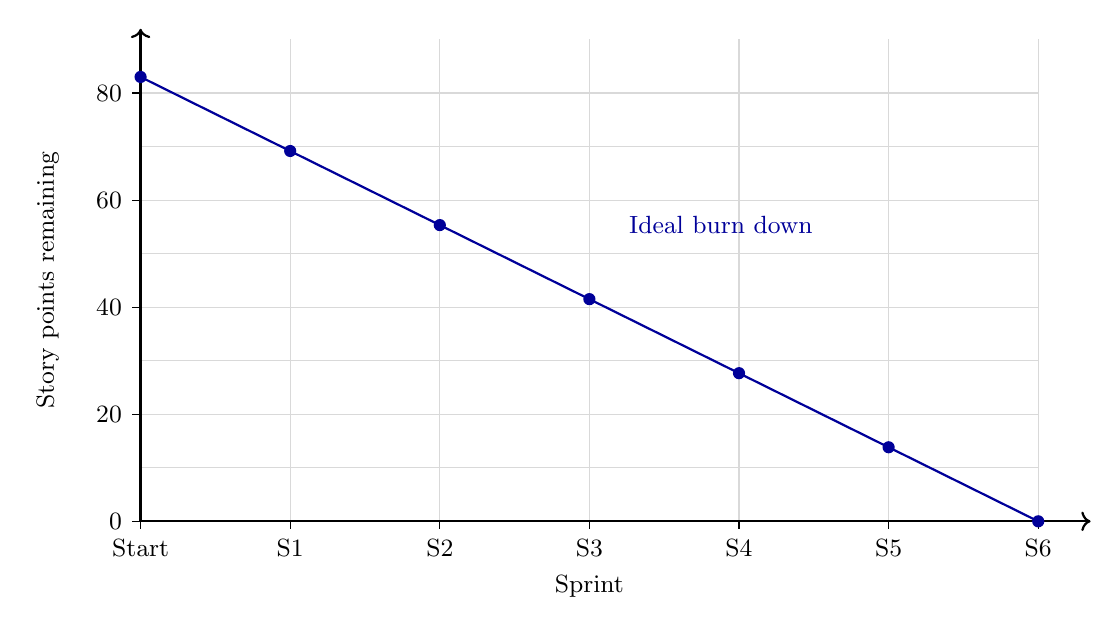
\begin{tikzpicture}[x=1.9cm,y=0.068cm,font=\small]
  % grid
  \foreach \y in {10,20,...,80} \draw[gray!30] (0,\y) -- (6,\y);
  \foreach \x in {1,...,6} \draw[gray!30] (\x,0) -- (\x,90);
  % axes
  \draw[->,thick] (0,0) -- (6.35,0);
  \draw[->,thick] (0,0) -- (0,92);
  \foreach \x/\l in {0/Start,1/S1,2/S2,3/S3,4/S4,5/S5,6/S6}
    \draw (\x,0) -- (\x,-1.5) node[below] {\l};
  \foreach \y in {0,20,40,60,80}
    \draw (0,\y) -- (-0.06,\y) node[left] {\y};
  \node[below=16pt] at (3,0) {Sprint};
  \node[rotate=90] at (-0.62,45) {Story points remaining};
  % ideal line
  \draw[thick,blue!60!black] (0,83) -- (6,0);
  \foreach \x/\y in {0/83.00,1/69.17,2/55.33,3/41.50,4/27.67,5/13.83,6/0.00}
    \fill[blue!60!black] (\x,\y) circle (2.2pt);
  \node[above right,blue!60!black] at (3.2,52) {Ideal burn down};
\end{tikzpicture}
\caption{Ideal burn down chart of InterfaceGuard}
\label{fig:burndown}
\end{figure}

\clearpage
 
% ============================================================
% CHAPTER 5: SYSTEM DESIGN
% ============================================================
\section{SYSTEM DESIGN}
 
\begin{spacing}{1.5}
\justifying
This chapter presents the design of InterfaceGuard. It explains the
technologies and the Model--View--Controller (MVC) framework on which the
system is organised, and it describes each module of the system in terms of
its purpose, inputs, processing and outputs.
\end{spacing}
 
% ------------------------------------------------------------
\subsection{Technology / Framework [MVC]}
 
% ------------------------------------------------------------
\subsubsection{Model--View--Controller Architecture}
 
\begin{spacing}{1.5}
\justifying
InterfaceGuard is organised according to the Model--View--Controller (MVC)
pattern, which separates the data and logic of an application (the Model),
what the user sees (the View) and the component that connects the two (the
Controller). This separation lets each part be developed, tested and changed
independently. Figure~\ref{fig:mvc} shows how the pattern is applied, and the
table below summarises the mapping.
\end{spacing}
 
\begin{figure}[H]
\centering
\resizebox{\linewidth}{!}{%
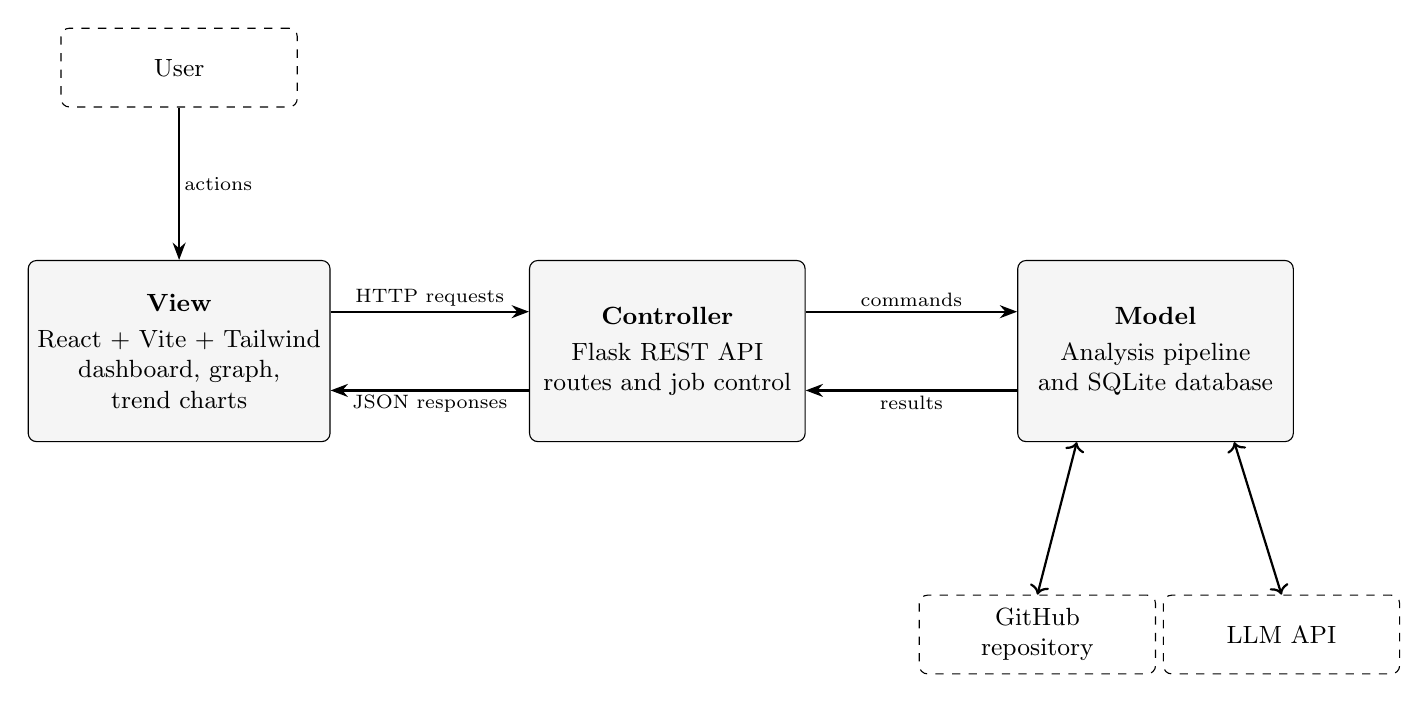
\begin{tikzpicture}[
  node distance=18mm,
  comp/.style={draw,rounded corners=3pt,align=center,font=\small,
               minimum width=3.5cm,minimum height=2.3cm,fill=gray!8},
  ext/.style={draw,dashed,rounded corners=3pt,align=center,font=\small,
              minimum width=3.0cm,minimum height=1cm},
  arr/.style={-{Stealth[length=2.2mm]},thick},
  lab/.style={font=\scriptsize,align=center,fill=white,inner sep=1.5pt}
]
\node[comp] (view) at (0,0) {\textbf{View}\\[2pt]React + Vite + Tailwind\\dashboard, graph,\\trend charts};
\node[comp] (ctrl) at (6.2,0) {\textbf{Controller}\\[2pt]Flask REST API\\routes and job control};
\node[comp] (model) at (12.4,0) {\textbf{Model}\\[2pt]Analysis pipeline\\and SQLite database};
\node[ext] (user) at (0,3.6) {User};
\node[ext] (gh) at (10.9,-3.6) {GitHub\\repository};
\node[ext] (llm) at (14.0,-3.6) {LLM API};
 
\draw[arr] (user) -- node[lab,right]{actions} (view);
\draw[arr] ([yshift=0.5cm]view.east) -- node[lab,above]{HTTP requests} ([yshift=0.5cm]ctrl.west);
\draw[arr] ([yshift=-0.5cm]ctrl.west) -- node[lab,below]{JSON responses} ([yshift=-0.5cm]view.east);
\draw[arr] ([yshift=0.5cm]ctrl.east) -- node[lab,above]{commands} ([yshift=0.5cm]model.west);
\draw[arr] ([yshift=-0.5cm]model.west) -- node[lab,below]{results} ([yshift=-0.5cm]ctrl.east);
\draw[arr,<->] ([xshift=-1.0cm]model.south) -- (gh.north);
\draw[arr,<->] ([xshift=1.0cm]model.south) -- (llm.north);
\end{tikzpicture}}
\caption{MVC architecture of InterfaceGuard}
\label{fig:mvc}
\end{figure}
 
\begin{table}[H]
\centering
\renewcommand{\arraystretch}{1.5}
\setlength{\tabcolsep}{6pt}
 
\begin{tabular}{|L{1.1in}|L{2.1in}|L{2.15in}|}
\hline
\textbf{MVC Component} & \textbf{Implementation} & \textbf{Responsibility} \\
\hline
Model & Python analysis modules (JavaParser, PyDriller, NetworkX, ruptures) and the SQLite database & Holds the data and business logic: parsing, metrics, detection, scoring, history analysis and storage of results \\
\hline
View & React, Vite and Tailwind CSS dashboard with Recharts and React Flow & Displays the repository input page, overview, interface details, dependency graph and trend charts, and offers the PDF report \\
\hline
Controller & Flask REST API & Receives requests from the View, starts and controls analysis jobs, reads the Model and returns JSON results \\
\hline
\end{tabular}
\end{table}
 
% ------------------------------------------------------------
\subsubsection{Technologies Used}
 
\begin{spacing}{1.5}
\justifying
Every technology in the system is free and open-source. The table below lists
the technologies by role, and the reasons for choosing them follow.
\end{spacing}
 
\begin{table}[H]
\centering
\renewcommand{\arraystretch}{1.5}
\setlength{\tabcolsep}{6pt}
 
\begin{tabular}{|L{1.3in}|L{2.0in}|L{2.05in}|}
\hline
\textbf{Role} & \textbf{Technology} & \textbf{Purpose} \\
\hline
Analysed language & Java & Language of the repositories that are analysed \\
\hline
Analysis and backend language & Python & Analysis scripts and the backend application \\
\hline
Source code parsing & JavaParser, JavaSymbolSolver & Syntax trees and type resolution of Java code \\
\hline
Git history mining & PyDriller & Traversal of commits and their changes \\
\hline
Graph analysis & NetworkX & Dependency graph, cycle and coupling detection \\
\hline
Change-point detection & ruptures, SciPy & Locating the commit at which erosion begins \\
\hline
AI module & Free-tier LLM API (e.g.\ Google Gemini) & Explanations and refactoring recommendations \\
\hline
Backend framework & Flask & REST API and job control (Controller) \\
\hline
Database & SQLite & Storage of results and cached AI responses \\
\hline
Frontend & React, Vite, Tailwind CSS & Dashboard (View) \\
\hline
Visualisation & Recharts, React Flow / D3 & Trend charts and dependency graph \\
\hline
Reporting & WeasyPrint & PDF report generated from templates \\
\hline
Version control & Git, GitHub & Source management and repository input \\
\hline
\end{tabular}
\end{table}
 
\begin{spacing}{1.5}
\justifying
\begin{itemize}[leftmargin=*,itemsep=2pt]
  \item \textbf{Python} offers mature libraries for Git mining, graph analysis
        and change-point detection, and it connects easily to LLM APIs.
  \item \textbf{JavaParser} removes the need for a custom Java parser and, with
        JavaSymbolSolver, resolves types across files, which is needed to find
        implementing classes and dependencies.
  \item \textbf{Flask} is a small framework that suits a REST API with a few
        routes and runs on a personal laptop.
  \item \textbf{SQLite} needs no separate installation and is sufficient for
        a single-user prototype.
  \item \textbf{React with Vite and Tailwind CSS} gives a fast, component-based
        interface, and Recharts and React Flow supply ready-made charts and
        graph components.
\end{itemize}
\end{spacing}
 
% ------------------------------------------------------------
\subsubsection{Main API Routes}
 
\begin{spacing}{1.5}
\justifying
The Controller exposes the following main routes to the View.
\end{spacing}
 
\begin{table}[H]
\centering
\renewcommand{\arraystretch}{1.5}
\setlength{\tabcolsep}{6pt}
 
\begin{tabular}{|L{0.7in}|L{2.35in}|L{2.3in}|}
\hline
\textbf{Method} & \textbf{Route} & \textbf{Purpose} \\
\hline
POST & /api/analyze & Submit a GitHub URL and start an analysis \\
\hline
GET & /api/analysis/\{id\}/status & Report the progress of a running analysis \\
\hline
GET & /api/analysis/\{id\}/overview & Erosion Index, severity distribution, most eroded interfaces \\
\hline
GET & /api/analysis/\{id\}/interfaces/\{name\} & Details, trend and AI explanation of one interface \\
\hline
GET & /api/analysis/\{id\}/graph & Dependency graph with cycles and coupled nodes \\
\hline
GET & /api/analysis/\{id\}/report & Download the PDF report \\
\hline
\end{tabular}
\end{table}
 
% ------------------------------------------------------------
\subsection{Module Description}
 
\begin{spacing}{1.5}
\justifying
InterfaceGuard consists of nine modules. The first six form the Model's
analysis pipeline, the seventh holds the Controller and storage, and the last
two are the View and the report generator. For each module, the input,
processing and output are described below.
\end{spacing}
 
% ------------------------------------------------------------
\Needspace{12\baselineskip}
\subsubsection{Repository Import and Parsing Module}
 
\begin{spacing}{1.5}
\justifying
This module acquires the Java repository and converts its source code into a structure that the other modules can analyse.
 
\begin{itemize}[leftmargin=*,itemsep=2pt]
  \item \textbf{Input:} a public GitHub repository URL.
  \item \textbf{Processing:} the repository is cloned and its URL validated. JavaParser builds the syntax tree of every Java source file, and JavaSymbolSolver resolves types. From the trees, each interface, its methods and its implementing classes are extracted. PyDriller reads the Git log so that the same extraction can be repeated at selected commits.
  \item \textbf{Output:} interface snapshots (name, methods, implementers, commit) for each analysed commit.
\end{itemize}
\end{spacing}
 
% ------------------------------------------------------------
\Needspace{12\baselineskip}
\subsubsection{Metrics Module}
 
\begin{spacing}{1.5}
\justifying
This module measures the design of each interface at each commit.
 
\begin{itemize}[leftmargin=*,itemsep=2pt]
  \item \textbf{Input:} interface snapshots.
  \item \textbf{Processing:} the Chidamber--Kemerer metrics (CBO, LCOM, RFC, WMC, DIT, NOC) are computed and aggregated over the implementers of the interface. The erosion metrics are computed from the history: method-count growth, interface churn across commits, breaking change count (removed or renamed methods that would break implementers) and interface cohesion (whether clients use only a subset of the interface).
  \item \textbf{Output:} a set of CK and erosion metric values for every interface snapshot.
\end{itemize}
\end{spacing}
 
% ------------------------------------------------------------
\Needspace{12\baselineskip}
\subsubsection{Detection Module}
 
\begin{spacing}{1.5}
\justifying
This module finds the specific design problems that indicate erosion.
 
\begin{itemize}[leftmargin=*,itemsep=2pt]
  \item \textbf{Input:} interface snapshots and their metrics.
  \item \textbf{Processing:} ISP violations are detected by finding implementing classes with empty, no-operation or exception-throwing method bodies. A dependency graph of types and packages is built with NetworkX to detect cyclic dependencies and highly coupled classes. The code smells God Class, Large Class, Long Method, Feature Envy, Refused Bequest and Fat Interface are detected using documented metric thresholds.
  \item \textbf{Output:} a list of violations, cycles and smells for each interface snapshot.
\end{itemize}
\end{spacing}
 
% ------------------------------------------------------------
\Needspace{12\baselineskip}
\subsubsection{Scoring Module}
 
\begin{spacing}{1.5}
\justifying
This module turns the separate indicators into a single, comparable measure.
 
\begin{itemize}[leftmargin=*,itemsep=2pt]
  \item \textbf{Input:} metrics, violations, cycles and smells.
  \item \textbf{Processing:} the normalised indicators are combined into an Interface Health Score from 0 to 100 for each interface. The scores are aggregated, weighted by dependency count so that widely used interfaces count more, into a project-level Erosion Index. Each interface is assigned a severity class of Low, Medium, High or Critical.
  \item \textbf{Output:} a Health Score and severity class per interface and commit, and an Erosion Index per commit.
\end{itemize}
\end{spacing}
 
% ------------------------------------------------------------
\Needspace{12\baselineskip}
\subsubsection{History and Trend Module}
 
\begin{spacing}{1.5}
\justifying
This module adds the time dimension, and shows when erosion began and whether it is getting worse.
 
\begin{itemize}[leftmargin=*,itemsep=2pt]
  \item \textbf{Input:} the series of Health Scores of each interface across the analysed commits.
  \item \textbf{Processing:} change-point detection (CUSUM or PELT, using ruptures and SciPy) is applied to each series. This identifies the commit, author and date at which erosion begins, instead of relying on a fixed threshold. A rule-based erosion trend, computed from the recent slope of the Health Score and the change-point result, labels each interface as Stable, Rising or Accelerating.
  \item \textbf{Output:} the onset commit, author and date, and the trend label of each interface.
\end{itemize}
\end{spacing}
 
% ------------------------------------------------------------
\Needspace{12\baselineskip}
\subsubsection{AI Explanation Module}
 
\begin{spacing}{1.5}
\justifying
This module explains each flagged interface in plain language and recommends a fix.
 
\begin{itemize}[leftmargin=*,itemsep=2pt]
  \item \textbf{Input:} the method list, metrics and violation details of each flagged interface.
  \item \textbf{Processing:} the details are sent to a free-tier LLM API, which returns an explanation of why the interface is eroding and a concrete refactoring recommendation, such as splitting the interface into two smaller ones. The module checks that every method named in a suggestion actually exists in the interface, caches the response to stay within free-tier rate limits, and labels the output as AI-generated.
  \item \textbf{Output:} a validated explanation and refactoring recommendation for each flagged interface.
\end{itemize}
\end{spacing}
 
% ------------------------------------------------------------
\Needspace{12\baselineskip}
\subsubsection{Storage and API Module (Controller)}
 
\begin{spacing}{1.5}
\justifying
This module connects the dashboard to the analysis pipeline and keeps the results.
 
\begin{itemize}[leftmargin=*,itemsep=2pt]
  \item \textbf{Input:} requests from the dashboard and results from the analysis modules.
  \item \textbf{Processing:} the Flask backend starts an analysis job when a URL is submitted, runs the pipeline, and writes the results and cached AI responses to SQLite. It then serves the stored results to the dashboard through the routes listed in Section~5.1.
  \item \textbf{Output:} JSON responses to the dashboard and the stored analysis data.
\end{itemize}
\end{spacing}
 
% ------------------------------------------------------------
\Needspace{12\baselineskip}
\subsubsection{Dashboard Module (View)}
 
\begin{spacing}{1.5}
\justifying
This module presents the results to the user as an interactive web application built with React, Vite and Tailwind CSS.
 
\begin{itemize}[leftmargin=*,itemsep=2pt]
  \item \textbf{Input:} JSON data from the API and the user's actions.
  \item \textbf{Processing:} the dashboard has a repository input page, an analysis progress view, a project overview (Erosion Index, severity distribution and most eroded interfaces), and a per-interface detail view with metrics, violations, smells, trend, onset commit and the AI explanation. Recharts draws trend charts of metrics, Health Scores and the Erosion Index across commits with change-point markers, and React Flow draws an interactive dependency graph that highlights cycles and tightly coupled nodes.
  \item \textbf{Output:} the interactive views, and a request for the PDF report when the user asks for it.
\end{itemize}
\end{spacing}
 
% ------------------------------------------------------------
\Needspace{12\baselineskip}
\subsubsection{Report Module}
 
\begin{spacing}{1.5}
\justifying
This module produces a document that the user can keep and share.
 
\begin{itemize}[leftmargin=*,itemsep=2pt]
  \item \textbf{Input:} the stored findings of an analysis.
  \item \textbf{Processing:} a report template is filled with the Erosion Index, the most eroded interfaces, their trends and the AI recommendations, and WeasyPrint converts it to a PDF file.
  \item \textbf{Output:} a downloadable PDF report.
\end{itemize}
\end{spacing}
 
 
\clearpage


% ============================================================
% CHAPTER 6: CODING
% ============================================================
\section{CODING}

\begin{spacing}{1.5}
\justifying
To ensure maintainability, readability, and architectural consistency across both the Python backend and the React frontend, strict coding standards were adopted throughout the development of InterfaceGuard. This chapter outlines the development conventions, architectural rules, and verified source code implementations representing the core modules of the software.
\end{spacing}

% ------------------------------------------------------------
\subsection{Coding Standards Used in the Project}

\begin{spacing}{1.3}
\justifying

\textbf{1. General Coding Practices}
\begin{itemize}[leftmargin=*,itemsep=3pt,topsep=3pt]
    \item \textbf{Modularity:} Every analyzer module encapsulates a single responsibility, isolating syntax parsing from metric computation and scoring.
    \item \textbf{Descriptive Naming:} Identifiers strictly follow domain terminology (e.g., \texttt{InterfaceSnapshot}, \texttt{isp\_violations}, \texttt{health\_score}).
    \item \textbf{Consistent Formatting:} Python code adheres to four-space indentation, while JavaScript and TypeScript use standard two-space indentation.
\end{itemize}

\textbf{2. Frontend Standards (React, Tailwind CSS, JavaScript)}
\begin{itemize}[leftmargin=*,itemsep=3pt,topsep=3pt]
    \item React functional components with Hooks (\texttt{useState}, \texttt{useEffect}, \texttt{useMemo}) are used exclusively.
    \item Styling adheres strictly to Tailwind CSS utility tokens based on the Software Architecture Field Journal theme (\#2E4036 Forest Green, \#CC5833 Clay, \#F2F0E9 Cream).
    \item Component files use PascalCase (e.g., \texttt{Overview.tsx}, \texttt{InterfaceDetail.tsx}, \texttt{DependencyGraph.tsx}), while utility functions use camelCase.
\end{itemize}

\textbf{3. Backend Standards (Python Flask)}
\begin{itemize}[leftmargin=*,itemsep=3pt,topsep=3pt]
    \item Adheres strictly to the PEP 8 style guide for Python code formatting.
    \item Every module and public function includes descriptive docstrings detailing arguments, return types, and exceptions.
    \item Deterministic error handling: all route handlers wrap pipeline calls in \texttt{try-except} blocks and return standardized JSON error envelopes.
\end{itemize}

\textbf{4. Database Standards (SQLite \& MongoDB)}
\begin{itemize}[leftmargin=*,itemsep=3pt,topsep=3pt]
    \item Relational SQLite models enforce foreign-key constraints linking repositories, commits, and interface snapshots.
    \item High-frequency lookup fields (\texttt{repository\_id}, \texttt{commit\_hash}, \texttt{name}) are explicitly indexed for rapid query retrieval.
    \item Raw AST dumps and exploratory analysis logs are stored in flexible MongoDB document collections.
\end{itemize}

\textbf{5. Security and Quality Standards}
\begin{itemize}[leftmargin=*,itemsep=3pt,topsep=3pt]
    \item Repository URLs and paths are strictly validated before subprocess execution to prevent shell command injection.
    \item Sensitive credentials, including Gemini API keys, are loaded via environment variables (\texttt{.env}) and excluded from version control.
    \item Parameterized SQL queries via SQLAlchemy prevent SQL injection vulnerabilities.
\end{itemize}

\end{spacing}

% ---------- STANDARDS SUMMARY TABLE (ALIGNED) ----------
\begin{table}[H]
\centering
\caption{Summary of Coding Standards and Quality Improvements}
\label{tab:coding_standards}
\renewcommand{\arraystretch}{1.35}
\setlength{\tabcolsep}{6pt}
\small

\begin{tabularx}{\linewidth}{|>{\raggedright\arraybackslash}p{1.4in}|Y|Y|}
\hline
\textbf{Area} & \textbf{Followed Standard} & \textbf{Recommended Improvement} \\
\hline
Python Backend & PEP 8, Flask Application Factory, Blueprint isolation & Add automated static type verification with mypy. \\
\hline
React Frontend & React 18/19 functional components, Tailwind CSS & Migrate all legacy components to strict TypeScript. \\
\hline
Database & SQLite relational schema with foreign key cascades & Implement connection pooling for concurrent audit runs. \\
\hline
API Design & RESTful JSON endpoints with status codes & Generate interactive OpenAPI / Swagger specifications. \\
\hline
Security & Environment secret management and path validation & Add IP-based rate limiting on repository intake endpoints. \\
\hline
\end{tabularx}
\end{table}

% ------------------------------------------------------------
\subsection{Project Coding}

\begin{spacing}{1.4}
\justifying
The following listings represent the authentic, verified source code implementations from the core modules of InterfaceGuard.
\end{spacing}

% ------------------------------------------------------------
\subsubsection{Flask Application Initialization}

\begin{lstlisting}[language=Python]
import os
from flask import Flask
from flask_cors import CORS
from app.core.config import Config
from app.models import db

def create_app(config_overrides=None):
    app = Flask(__name__)
    app.config.from_object(Config)

    if config_overrides:
        app.config.update(config_overrides)

    Config.DATA_DIR.mkdir(parents=True, exist_ok=True)
    Config.REPORTS_DIR.mkdir(parents=True, exist_ok=True)
    Config.TEMP_DIR.mkdir(parents=True, exist_ok=True)

    db.init_app(app)
    CORS(app, resources={r'/*': {'origins': '*'}})

    from app.routes.repository_routes import repository_bp
    app.register_blueprint(repository_bp)

    from app.api.api_v1 import api_v1_bp
    app.register_blueprint(api_v1_bp)

    with app.app_context():
        db.create_all()

    return app
\end{lstlisting}

\noindent\textit{Purpose:} Implements the Flask application factory pattern, binds the SQLAlchemy database, configures cross-origin resource sharing (CORS), and registers the versioned REST API blueprints.

% ------------------------------------------------------------
\subsubsection{Domain Models (Interface \& Snapshot)}

\begin{lstlisting}[language=Python]
from app.models import db
from datetime import datetime

class Interface(db.Model):
    __tablename__ = 'interfaces'
    id = db.Column(db.Integer, primary_key=True)
    repository_id = db.Column(db.Integer, db.ForeignKey('repositories.id'), nullable=False)
    name = db.Column(db.String(255), nullable=False)
    file_path = db.Column(db.String(512), nullable=False)
    package_name = db.Column(db.String(255))
    snapshots = db.relationship('InterfaceSnapshot', backref='interface', lazy=True)

class InterfaceSnapshot(db.Model):
    __tablename__ = 'interface_snapshots'
    id = db.Column(db.Integer, primary_key=True)
    interface_id = db.Column(db.Integer, db.ForeignKey('interfaces.id'), nullable=False)
    commit_hash = db.Column(db.String(40), nullable=False)
    commit_date = db.Column(db.DateTime, default=datetime.utcnow)
    method_count = db.Column(db.Integer, default=0)
    isp_violations_count = db.Column(db.Integer, default=0)
    cbo = db.Column(db.Float, default=0.0)
    lcom = db.Column(db.Float, default=0.0)
    health_score = db.Column(db.Float, default=100.0)
    is_eroding = db.Column(db.Boolean, default=False)
\end{lstlisting}

\noindent\textit{Purpose:} Defines the relational schema modeling tracked Java interfaces and their longitudinal commit snapshots containing CK metrics, ISP violation counts, and composite Health Scores.

% ------------------------------------------------------------
\subsubsection{JavaParser 3.26.2 AST Extraction Bridge}

\begin{lstlisting}[language=Python]
import json, logging, subprocess
from pathlib import Path
from app.core.config import Config

logger = logging.getLogger(__name__)

def parse_with_javaparser(paths: list[str]) -> dict:
    jar_path = Config.JAVAPARSER_JAR
    if not jar_path.exists():
        logger.warning('JavaParser bridge jar not found. Using fallback.')
        return parse_with_fallback(paths)

    optimized_paths = []
    for p in paths:
        src = Path(p) / 'src' / 'main' / 'java'
        optimized_paths.append(str(src) if src.exists() else str(p))

    cmd = ['java', '-jar', str(jar_path)] + optimized_paths
    proc = subprocess.run(cmd, capture_output=True, text=True, timeout=90)
    if proc.returncode == 0 and proc.stdout.strip():
        data = json.loads(proc.stdout.strip())
        data['parser_engine'] = 'JavaParser 3.26.2'
        return data
    return parse_with_fallback(paths)
\end{lstlisting}

\noindent\textit{Purpose:} Executes the JavaParser 3.26.2 abstract syntax tree extraction bridge via subprocess IPC, emitting JSON representations of interfaces, methods, and implementing class bodies.

% ------------------------------------------------------------
\subsubsection{Interface Segregation Principle (ISP) Violation Detector}

\begin{lstlisting}[language=Python]
def detect_isp_violations(interface_name, interface_methods, implementing_classes):
    findings = []
    iface_method_names = {m['name'] for m in interface_methods}

    for cls in implementing_classes:
        cls_name = cls.get('name', 'UnknownClass')
        file_path = cls.get('file_path', '')

        for m in cls.get('methods', []):
            m_name = m.get('name', '')
            if m_name not in iface_method_names:
                continue

            if m.get('is_exception_stub', False):
                findings.append({
                    'category': 'isp_violation',
                    'rule_name': 'Exception-Throwing Stub',
                    'severity': 'critical',
                    'class_name': cls_name,
                    'method_name': m_name,
                    'file_path': file_path,
                    'description': f'Class {cls_name} implements {interface_name} but throws an exception in {m_name}().'
                })
            elif m.get('is_empty', False):
                findings.append({
                    'category': 'isp_violation',
                    'rule_name': 'Empty Implementation Stub',
                    'severity': 'medium',
                    'class_name': cls_name,
                    'method_name': m_name,
                    'file_path': file_path,
                    'description': f'Class {cls_name} provides an empty body for {m_name}().'
                })
    return findings
\end{lstlisting}

\noindent\textit{Purpose:} Identifies concrete classes forced to implement hollow stubs or throw runtime exceptions (\texttt{UnsupportedOperationException}), establishing empirical evidence of ISP violations.

% ------------------------------------------------------------
\subsubsection{Composite Interface Health Scoring Formulation}

\begin{lstlisting}[language=Python]
DEFAULT_WEIGHTS = {
    'isp_violations': 0.30,
    'method_bloat': 0.20,
    'coupling': 0.15,
    'dependency_cycles': 0.15,
    'churn': 0.10,
    'cohesion': 0.10,
}

def compute_health_score(method_count, isp_count, total_methods, cbo, in_cycle, churn, breaking_changes, cohesion, weights=None):
    w = weights or DEFAULT_WEIGHTS
    denom = max(1, total_methods)
    isp_p = min(1.0, isp_count / float(denom))
    bloat_p = min(1.0, max(0, method_count - 4) / 8.0)
    coupling_p = min(1.0, float(cbo) / 8.0)
    cycle_p = 1.0 if in_cycle else 0.0
    churn_p = min(1.0, (float(churn) + float(breaking_changes) * 2.0) / 10.0)
    cohesion_p = max(0.0, min(1.0, 1.0 - float(cohesion)))

    total_penalty = (
        w['isp_violations'] * isp_p + w['method_bloat'] * bloat_p +
        w['coupling'] * coupling_p + w['dependency_cycles'] * cycle_p +
        w['churn'] * churn_p + w['cohesion'] * cohesion_p
    )
    score = round(max(0.0, min(100.0, 100.0 * (1.0 - total_penalty))), 1)
    severity = 'critical' if score < 40 else 'high' if score < 60 else 'warning' if score < 80 else 'healthy'
    return {'health_score': score, 'severity': severity, 'is_eroding': score < 70.0}
\end{lstlisting}

\noindent\textit{Purpose:} Combines ISP stubs, method bloat, coupling, cyclic dependencies, churn, and cohesion into a transparent, normalized 0 to 100 Health Score.

% ------------------------------------------------------------
\subsubsection{CUSUM Time-Series Change-Point \& Trend Detection}

\begin{lstlisting}[language=Python]
import numpy as np

def classify_erosion_trend(scores: list[float]) -> str:
    if len(scores) < 3:
        return 'stable'
    erosion_levels = [100.0 - s for s in scores]
    x = np.arange(len(erosion_levels))
    slope, _ = np.polyfit(x, erosion_levels, 1)
    if slope <= 1.5:
        return 'stable'
    if len(erosion_levels) >= 4:
        curvature = np.polyfit(x, erosion_levels, 2)[0]
        if curvature > 0.4:
            return 'accelerating'
    return 'rising'

def detect_change_points_cusum(commits: list[dict], scores: list[float], threshold: float = 12.0) -> list[dict]:
    if len(scores) < 3:
        return []
    change_points = []
    for i in range(1, len(scores)):
        drop = scores[i - 1] - scores[i]
        if drop >= threshold:
            commit = commits[i]
            change_points.append({
                'commit_hash': commit.get('commit_hash', ''),
                'commit_date': commit.get('commit_date'),
                'author': commit.get('author', 'unknown'),
                'drop_amount': round(drop, 1),
                'score_before': round(scores[i - 1], 1),
                'score_after': round(scores[i], 1)
            })
    return change_points
\end{lstlisting}

\noindent\textit{Purpose:} Applies polynomial curve fitting to classify erosion trends (\texttt{stable}, \texttt{rising}, \texttt{accelerating}) and detects structural degradation points where Health Scores drop by 12 points or more.

% ------------------------------------------------------------
\subsubsection{Directed Dependency Graph \& Cycle Analyzer}

\begin{lstlisting}[language=Python]
import networkx as nx

def build_dependency_graph(interfaces: list[dict], classes: list[dict]):
    G = nx.DiGraph()
    for iface in interfaces:
        G.add_node(iface['name'], node_type='interface', package=iface.get('package', ''))
    for cls in classes:
        G.add_node(cls['name'], node_type='class', package=cls.get('package', ''))
        for impl in cls.get('implements', []):
            G.add_edge(cls['name'], impl, relationship='implements')
        for ext in cls.get('extends', []):
            G.add_edge(cls['name'], ext, relationship='extends')

    cycles = list(nx.simple_cycles(G))
    return {
        'nodes': list(G.nodes(data=True)),
        'edges': list(G.edges(data=True)),
        'cycles': cycles
    }
\end{lstlisting}

\noindent\textit{Purpose:} Constructs a directed type graph using NetworkX to map inheritance and implementation edges, and isolates circular dependency loops across the system.

% ------------------------------------------------------------
\subsubsection{AI Explanation Engine \& Refactoring Validator}

\begin{lstlisting}[language=Python]
import hashlib, json, os
from app.core.config import Config

_EXPLANATION_CACHE = {}

def generate_explanation(interface_name, methods, implementing_classes, findings, metrics, use_llm=True):
    context = {'interface_name': interface_name, 'methods': methods, 'findings': findings, 'metrics': metrics}
    cache_key = hashlib.sha256(json.dumps(context, sort_keys=True).encode()).hexdigest()
    if cache_key in _EXPLANATION_CACHE:
        return _EXPLANATION_CACHE[cache_key]

    api_key = Config.GEMINI_API_KEY or os.getenv('GEMINI_API_KEY')
    if use_llm and api_key:
        try:
            explanation = _call_gemini_api(context, api_key)
            explanation = _validate_and_sanitize(explanation, methods)
            _EXPLANATION_CACHE[cache_key] = explanation
            return explanation
        except Exception:
            pass
    return generate_deterministic_fallback(context)
\end{lstlisting}

\noindent\textit{Purpose:} Queries the Google Gemini LLM API to produce natural-language explanations and verifies that all suggested method names exist in the AST, falling back to deterministic expert rules when offline.

% ------------------------------------------------------------
\subsubsection{React Overview Dashboard Component}

\begin{lstlisting}[language=JavaScript]
import React, { useEffect, useState } from 'react';
import { useParams } from 'react-router-dom';

export function Overview() {
  const { repoId } = useParams();
  const [data, setData] = useState(null);
  const [loading, setLoading] = useState(true);

  useEffect(() => {
    fetch(`/api/v1/repositories/${repoId}/overview`)
      .then((res) => res.json())
      .then((json) => {
        setData(json);
        setLoading(false);
      });
  }, [repoId]);

  if (loading) return <div className='p-8'>Auditing repository evolution...</div>;

  return (
    <div className='p-8 bg-[#F2F0E9] min-h-screen text-[#1A1A1A]'>
      <header className='mb-6 flex justify-between items-center border-b pb-4'>
        <h1 className='text-2xl font-bold font-serif text-[#2E4036]'>Architecture Field Journal</h1>
        <div className='px-4 py-2 rounded bg-white shadow font-mono'>
          Erosion Index: <span className='text-[#CC5833] font-bold'>{data.erosion_index}/100</span>
        </div>
      </header>
      <div className='grid grid-cols-3 gap-6'>
        <div className='bg-white p-6 rounded shadow border'>
          <h3 className='font-semibold text-gray-700'>Health Score</h3>
          <p className='text-4xl font-bold mt-2 text-[#2E4036]'>{data.average_health}/100</p>
        </div>
        <div className='bg-white p-6 rounded shadow border'>
          <h3 className='font-semibold text-gray-700'>Flagged Interfaces</h3>
          <p className='text-4xl font-bold mt-2 text-[#CC5833]'>{data.flagged_count}</p>
        </div>
        <div className='bg-white p-6 rounded shadow border'>
          <h3 className='font-semibold text-gray-700'>Dependency Cycles</h3>
          <p className='text-4xl font-bold mt-2 text-amber-600'>{data.cycle_count}</p>
        </div>
      </div>
    </div>
  );
}
\end{lstlisting}

\noindent\textit{Purpose:} Renders the React 19 overview dashboard, presenting repository Health Scores, eroding interface counts, and circular dependency statistics styled with the Field Journal theme.

\clearpage

% ============================================================ 
% CHAPTER 7: TESTING
% ============================================================ 
\section{TESTING}

\begin{spacing}{1.5}
\justifying
Testing validates that every stage of the InterfaceGuard pipeline operates reliably and accurately. The testing strategy focused on unit testing each independent analyzer using the Pytest framework alongside integration tests verifying end-to-end repository evaluation.
\end{spacing}

% ------------------------------------------------------------
\subsection{Unit Testing}

\begin{spacing}{1.5}
\justifying
A comprehensive suite of 43 unit tests was developed, validating repository ingestion, AST signature extraction, ISP violation pattern matching, metric computation, change-point detection, and PDF generation. Table~\ref{tab:testcases} details the primary unit test cases.
\end{spacing}

\begin{table}[htbp]
\centering
\caption{Unit test cases and execution outcomes}
\label{tab:testcases}
\renewcommand{\arraystretch}{1.4}
\setlength{\tabcolsep}{4pt}
\scriptsize
\begin{tabular}{|C{1.0cm}|L{1.8cm}|L{2.5cm}|L{2.8cm}|L{2.5cm}|C{1.1cm}|}
\hline
\textbf{Test ID} & \textbf{Module} & \textbf{Test Scenario} & \textbf{Input} & \textbf{Expected Output} & \textbf{Status} \\
\hline
TC01 & Validation & Ingest valid local Git path & Valid directory path & Validation success (True) & Pass \\
\hline
TC02 & Validation & Ingest invalid directory path & Non-existent path & Validation error (False) & Pass \\
\hline
TC03 & JavaParser & Parse interface declarations & Java file with 3 methods & Emits 3 method signatures & Pass \\
\hline
TC04 & JavaParser & Resolve implementing classes & Class implementing interface & Implements relationship recorded & Pass \\
\hline
TC05 & ISPDetector & Method throwing UnsupportedOp & Body throws UnsupportedOp & Flagged as ISP violation & Pass \\
\hline
TC06 & ISPDetector & Empty method body implementation & Empty method block \texttt{\{\}} & Flagged as empty body stub & Pass \\
\hline
TC07 & CKMetrics & Calculate CBO metric & Class referencing 5 types & CBO score computed as 5.0 & Pass \\
\hline
TC08 & CKMetrics & Calculate LCOM cohesion & Disjoint parameter methods & LCOM score accurately calculated & Pass \\
\hline
TC09 & Dependency & Detect circular dependency & A uses B, B uses A & Directed cycle flagged & Pass \\
\hline
TC10 & Scoring & Healthy interface evaluation & 0 stubs, low coupling & Health Score $\ge 80.0$ & Pass \\
\hline
TC11 & Scoring & Severely eroded interface & 5 stubs, high CBO, cyclic & Health Score $< 40.0$ & Pass \\
\hline
TC12 & ChangePoint & Detect sharp score drop & Health drops from 85 to 65 & Change-point recorded ($\Delta \ge 10$) & Pass \\
\hline
TC13 & AIExplainer & Offline fallback check & No Gemini API key & Returns rule-based advice & Pass \\
\hline
TC14 & AIExplainer & Method name verification & Recommendation text & Non-existent methods rejected & Pass \\
\hline
TC15 & Report & PDF report generation & Stored analysis findings & Valid PDF file emitted & Pass \\
\hline
\end{tabular}
\end{table}

\clearpage

% ============================================================ 
% CHAPTER 8: IMPLEMENTATION
% ============================================================ 
\section{IMPLEMENTATION}

\subsection{Implementation Method Used in Project}
\begin{spacing}{1.5}
\justifying
InterfaceGuard was implemented using the \textbf{Incremental Development Methodology}, aligning with the six two-week Scrum sprints. This allowed each component of the pipeline to be built, tested, and refined independently before being coupled to dependent modules.

\textbf{1. Requirement Analysis and Planning:} Detailed requirements were gathered by examining open-source Java projects to identify real-world manifestations of interface bloat and ISP violations. These findings were formalized into user stories and assigned story point estimates.

\textbf{2. Modular Design and Development:}
\begin{itemize}[leftmargin=*,itemsep=2pt]
  \item \textbf{AST Parsing Bridge:} Implemented using JavaParser 3.26.2 and packaged into an executable shaded jar with fallback support through Python's \texttt{javalang} library.
  \item \textbf{Git Mining Service:} Integrated PyDriller to traverse commit histories, checking out repository snapshots into memory.
  \item \textbf{Metrics and Anomaly Engine:} Built separate Python modules for CK metrics, parameter cohesion, ISP stub matching, and CUSUM analysis.
  \item \textbf{REST Controller and Dashboard:} Developed Flask API routes and the React single-page frontend.
\end{itemize}

\textbf{3. Testing and Debugging:} Iterative testing accompanied development. Flask's built-in debugger, browser developer tools, and Pytest test fixtures were utilized to diagnose AST tokenization errors and React Flow rendering issues.

\textbf{4. Deployment:} The backend runs locally on a Flask server connecting to SQLite, while the React frontend is compiled using Vite. The application is container-ready via Docker for reproducible deployments.

\textbf{5. Maintenance and Continuous Improvement:} Threshold calibration is performed against established Java benchmarks (such as Spring Framework and Apache Kafka) to ensure consistent scoring sensitivity.
\end{spacing}

\clearpage

% ============================================================ 
% CHAPTER 9: BUSINESS PERSPECTIVE
% ============================================================ 
\section{BUSINESS PERSPECTIVE}

\begin{spacing}{1.5}
\justifying
\textbf{Strategic Alignment and Market Relevance:} Software maintenance routinely accounts for 60\% to 80\% of total software lifecycle expenditure. By identifying structural interface decay during development rather than in production, InterfaceGuard significantly curtails long-term maintenance costs.

\textbf{Value Proposition:}
\begin{itemize}[leftmargin=*,itemsep=2pt]
  \item \textbf{Early Erosion Detection:} Locates the exact historical commit where design decay began, preventing compounding technical debt.
  \item \textbf{Actionable Architectural Advice:} Converts opaque metric scores into concrete, plain-language refactoring blueprints.
  \item \textbf{Zero Financial Cost:} Built entirely on free and open-source technologies, making enterprise-grade auditing accessible to students, startups, and small development teams.
\end{itemize}

\textbf{Operational Impact:} Incorporating InterfaceGuard into automated continuous integration (CI/CD) pipelines provides automated architectural governance, ensuring pull requests that violate the Interface Segregation Principle are caught before being merged.

\textbf{Competitive Advantage:} While existing tools like SonarQube or PMD assess static code snapshots, InterfaceGuard uniquely reconstructs evolutionary trajectories across Git commit histories, detects semantic ISP stubs, and synthesizes AI refactoring plans.

\textbf{Future Scalability and Commercial Potential:} The platform can expand into a cloud-hosted Software-as-a-Service (SaaS) model, offering GitHub App marketplace integrations, organization-wide architecture health dashboards, and automated refactoring pull request bots.

\textbf{Risk Mitigation:} Identifies undocumented dependency cycles and tightly coupled interfaces, mitigating key-person dependency risks across legacy systems.
\end{spacing}

\clearpage

% ============================================================ 
% CHAPTER 10: FUTURE SCOPE OR ENHANCEMENTS
% ============================================================ 
\section{FUTURE SCOPE OR ENHANCEMENTS}

\begin{spacing}{1.5}
\justifying
While the current version of InterfaceGuard provides an end-to-end interface erosion audit pipeline, several enhancements are planned for future iterations:

\begin{itemize}[leftmargin=*,itemsep=3pt]
  \item \textbf{AI-Based Personalization and Automated Refactoring PRs:} Fine-tuning LLMs on internal team code styles to automatically open GitHub Pull Requests that segregate bloated interfaces into cohesive role contracts.
  \item \textbf{Multi-Language AST Support:} Expanding the AST parsing bridge beyond Java to audit interfaces in TypeScript, C\#, Go, and Kotlin.
  \item \textbf{Advanced Communication and Collaboration Tools:} Integrating real-time architecture review rooms, team annotations, and Slack/Teams alert webhooks when an interface's health score drops.
  \item \textbf{Mobile Application Integration:} Developing lightweight Android and iOS companion apps for engineering managers to inspect build health scores and critical alerts on the go.
  \item \textbf{Role-Based Access Control and Security Enhancements:} Introducing SAML 2.0 / OAuth2 single sign-on (SSO) with fine-grained team permissions.
  \item \textbf{Cloud Integration and Scalability:} Migrating worker execution to Kubernetes clusters using Celery and Redis to audit enterprise repositories with tens of thousands of commits in parallel.
  \item \textbf{Blockchain-Based Skill / Audit Validation:} Generating verifiable, tamper-proof architectural compliance certificates on decentralized ledgers.
\end{itemize}
\end{spacing}

\clearpage

% ============================================================ 
% CHAPTER 11: APPENDIX
% ============================================================ 
\section{APPENDIX}

\subsection{Git History [Sprint Wise]}
\begin{spacing}{1.5}
\justifying
The repository's commit history confirms the incremental delivery of features across the six project sprints:
\begin{itemize}[leftmargin=*,itemsep=2pt]
  \item \textbf{Sprint 1 (\texttt{v0.1.0}):}
        \texttt{feat: initialize Flask backend framework};
        \texttt{feat: create SQLite schema for repositories and snapshots};
        \texttt{feat: implement repository URL validation}.
  \item \textbf{Sprint 2 (\texttt{v0.2.0}):}
        \texttt{feat: integrate PyDriller commit history walker};
        \texttt{feat: build JavaParser AST extraction bridge};
        \texttt{feat: extract interface method signatures and implementers}.
  \item \textbf{Sprint 3 (\texttt{v0.3.0}):}
        \texttt{feat: implement ISP violation detector for stub bodies};
        \texttt{feat: compute CK metrics (CBO, LCOM, RFC, WMC)};
        \texttt{feat: calculate interface churn and breaking changes}.
  \item \textbf{Sprint 4 (\texttt{v0.4.0}):}
        \texttt{feat: implement composite Interface Health Score formula};
        \texttt{feat: implement CUSUM time-series change-point detector};
        \texttt{feat: assign erosion severity and trend classifications}.
  \item \textbf{Sprint 5 (\texttt{v0.5.0}):}
        \texttt{feat: integrate Gemini LLM explanation API with cache};
        \texttt{feat: implement method validation on AI suggestions};
        \texttt{feat: build React overview dashboard and interface table}.
  \item \textbf{Sprint 6 (\texttt{v1.0.0}):}
        \texttt{feat: build interactive React Flow dependency graph};
        \texttt{feat: generate publication PDF reports via WeasyPrint};
        \texttt{test: complete 43 automated backend tests}.
\end{itemize}
\end{spacing}

\clearpage

\subsection{Screen Shots of Forms, Reports, Diagrams}
\begin{spacing}{1.5}
\justifying
The operational prototype features five core user interfaces and diagnostic visualizers, presented in Figures~\ref{fig:screen_landing} through~\ref{fig:screen_graph_side}.
\end{spacing}

\begin{figure}[H]
\centering
\IfFileExists{screenshots/landing-1440px.png}{%
  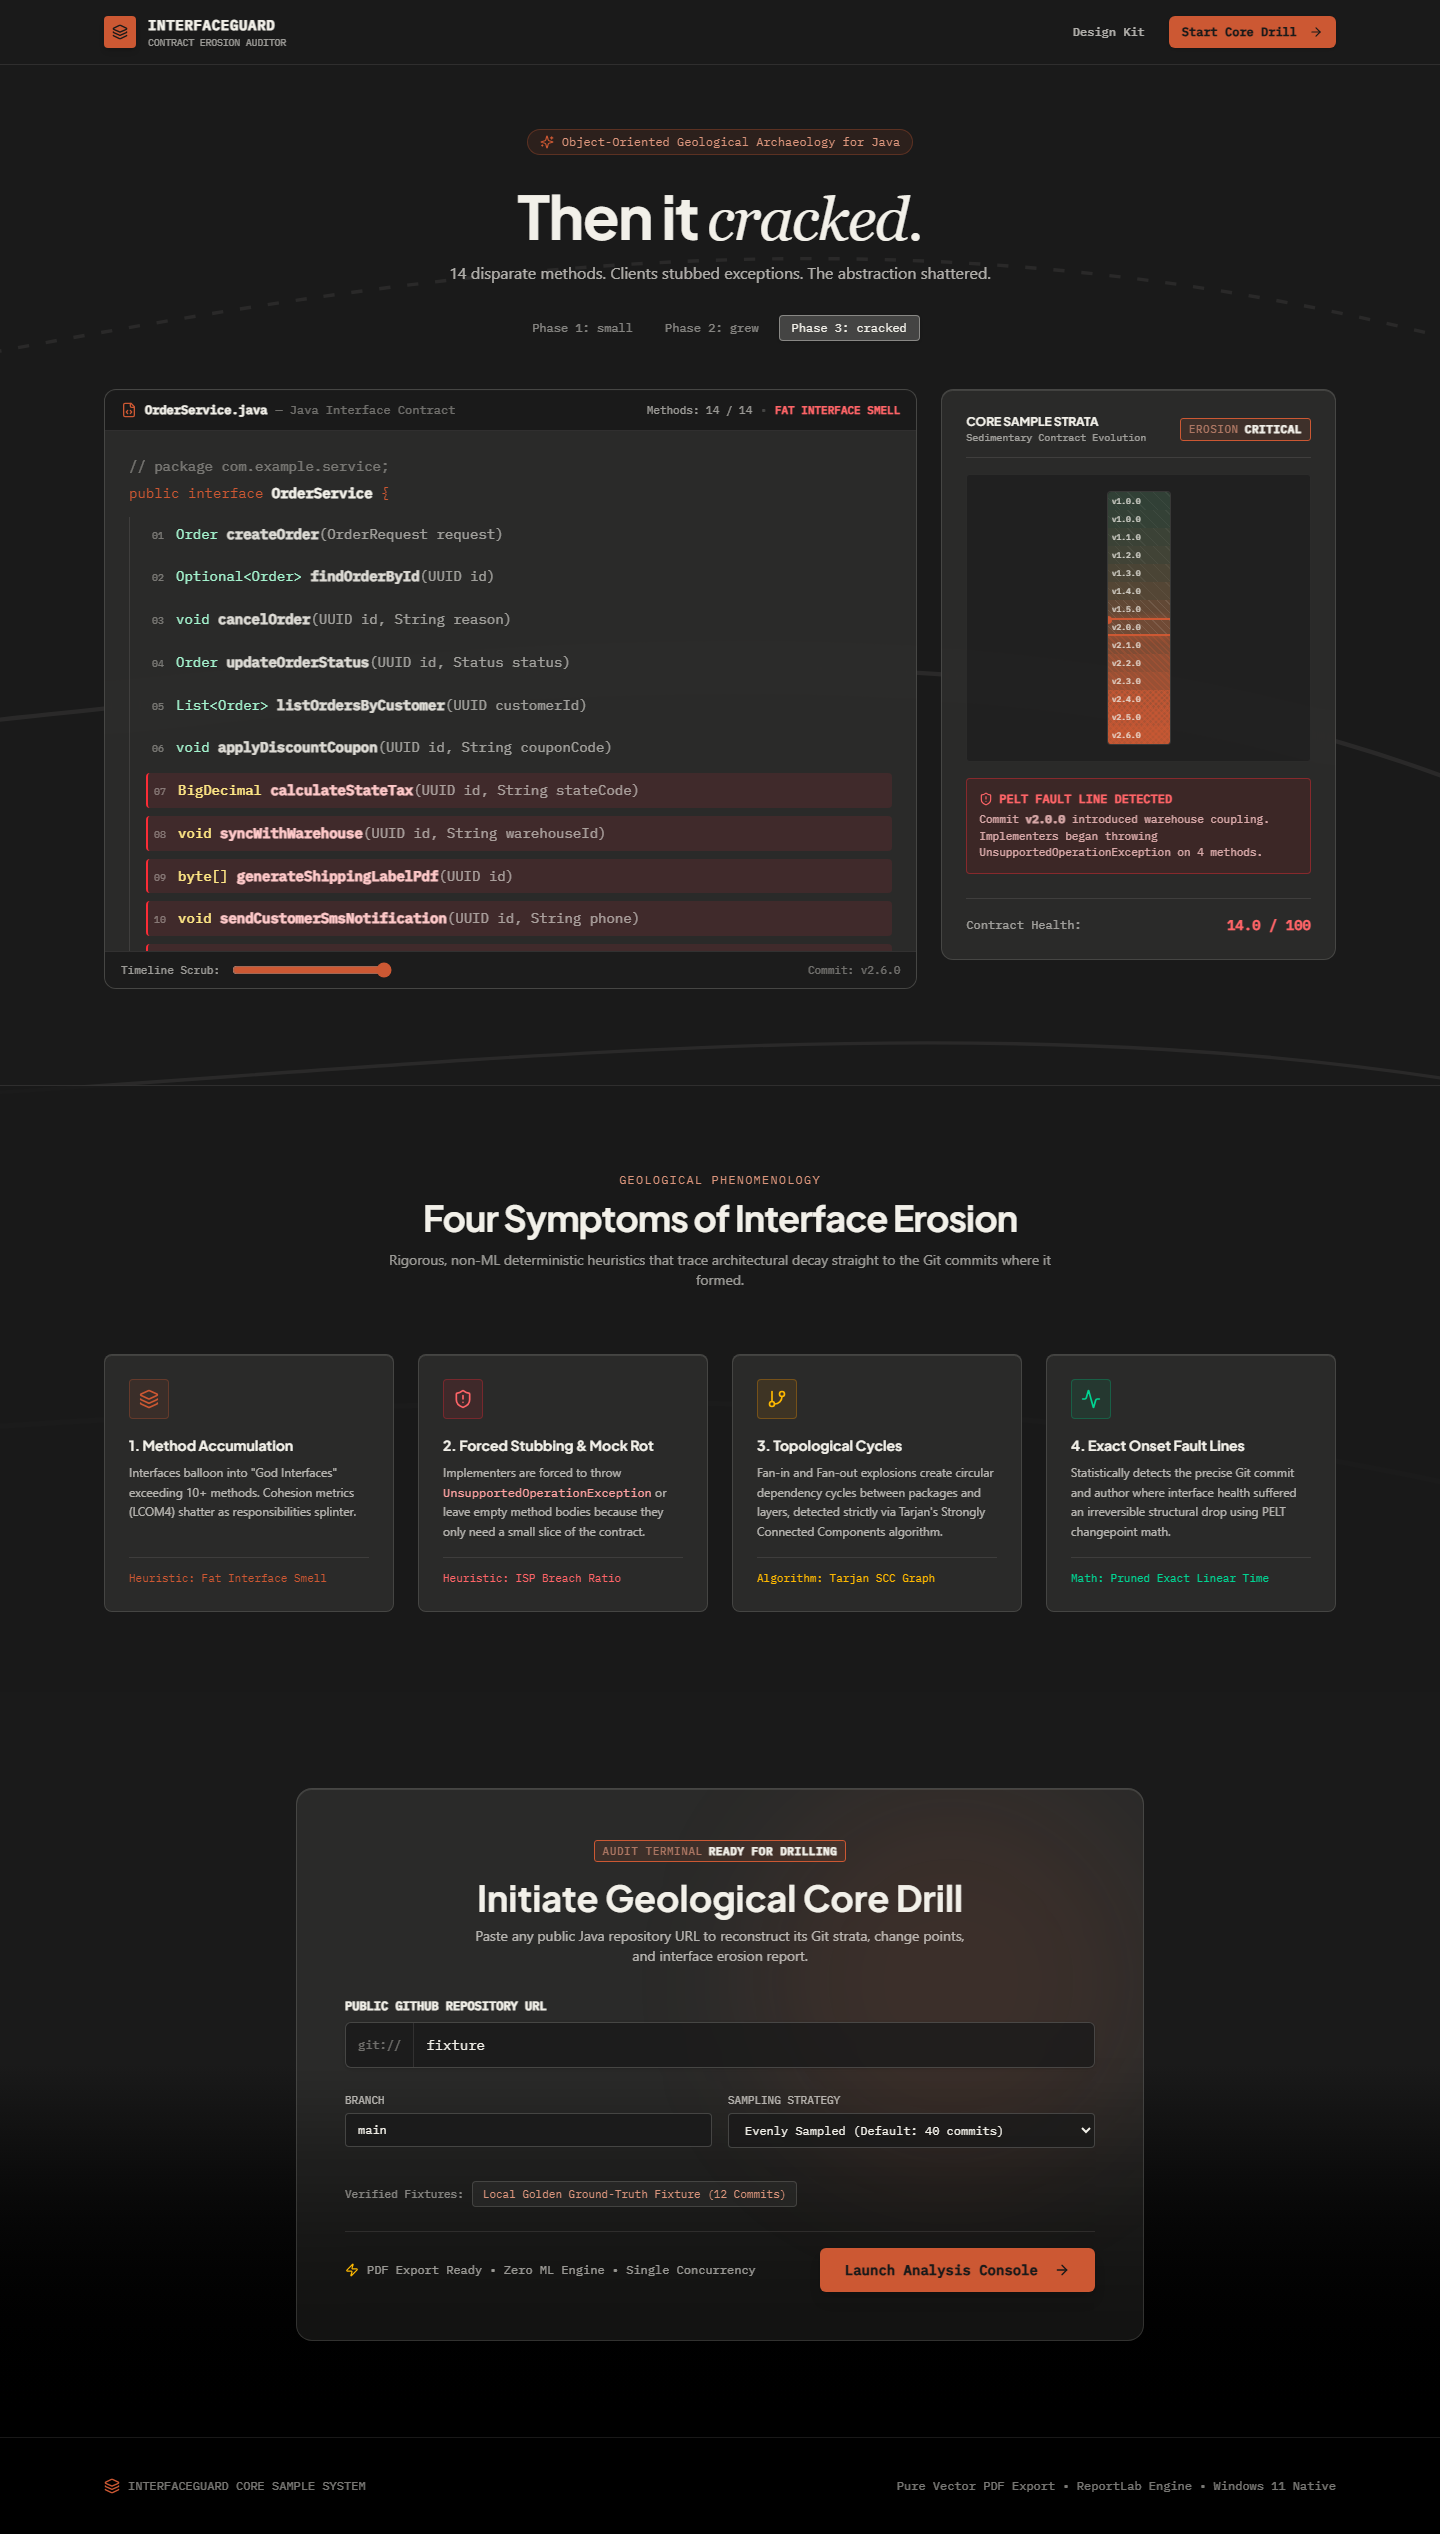
\includegraphics[width=0.92\textwidth]{screenshots/landing-1440px.png}%
}{%
  \fbox{\parbox[c][2.4in][c]{0.92\textwidth}{\centering\small Repository Intake and Configuration View}}%
}
\caption{Repository Intake and Configuration Launch Screen}
\label{fig:screen_landing}
\end{figure}

\begin{figure}[H]
\centering
\IfFileExists{screenshots/overview-1440px.png}{%
  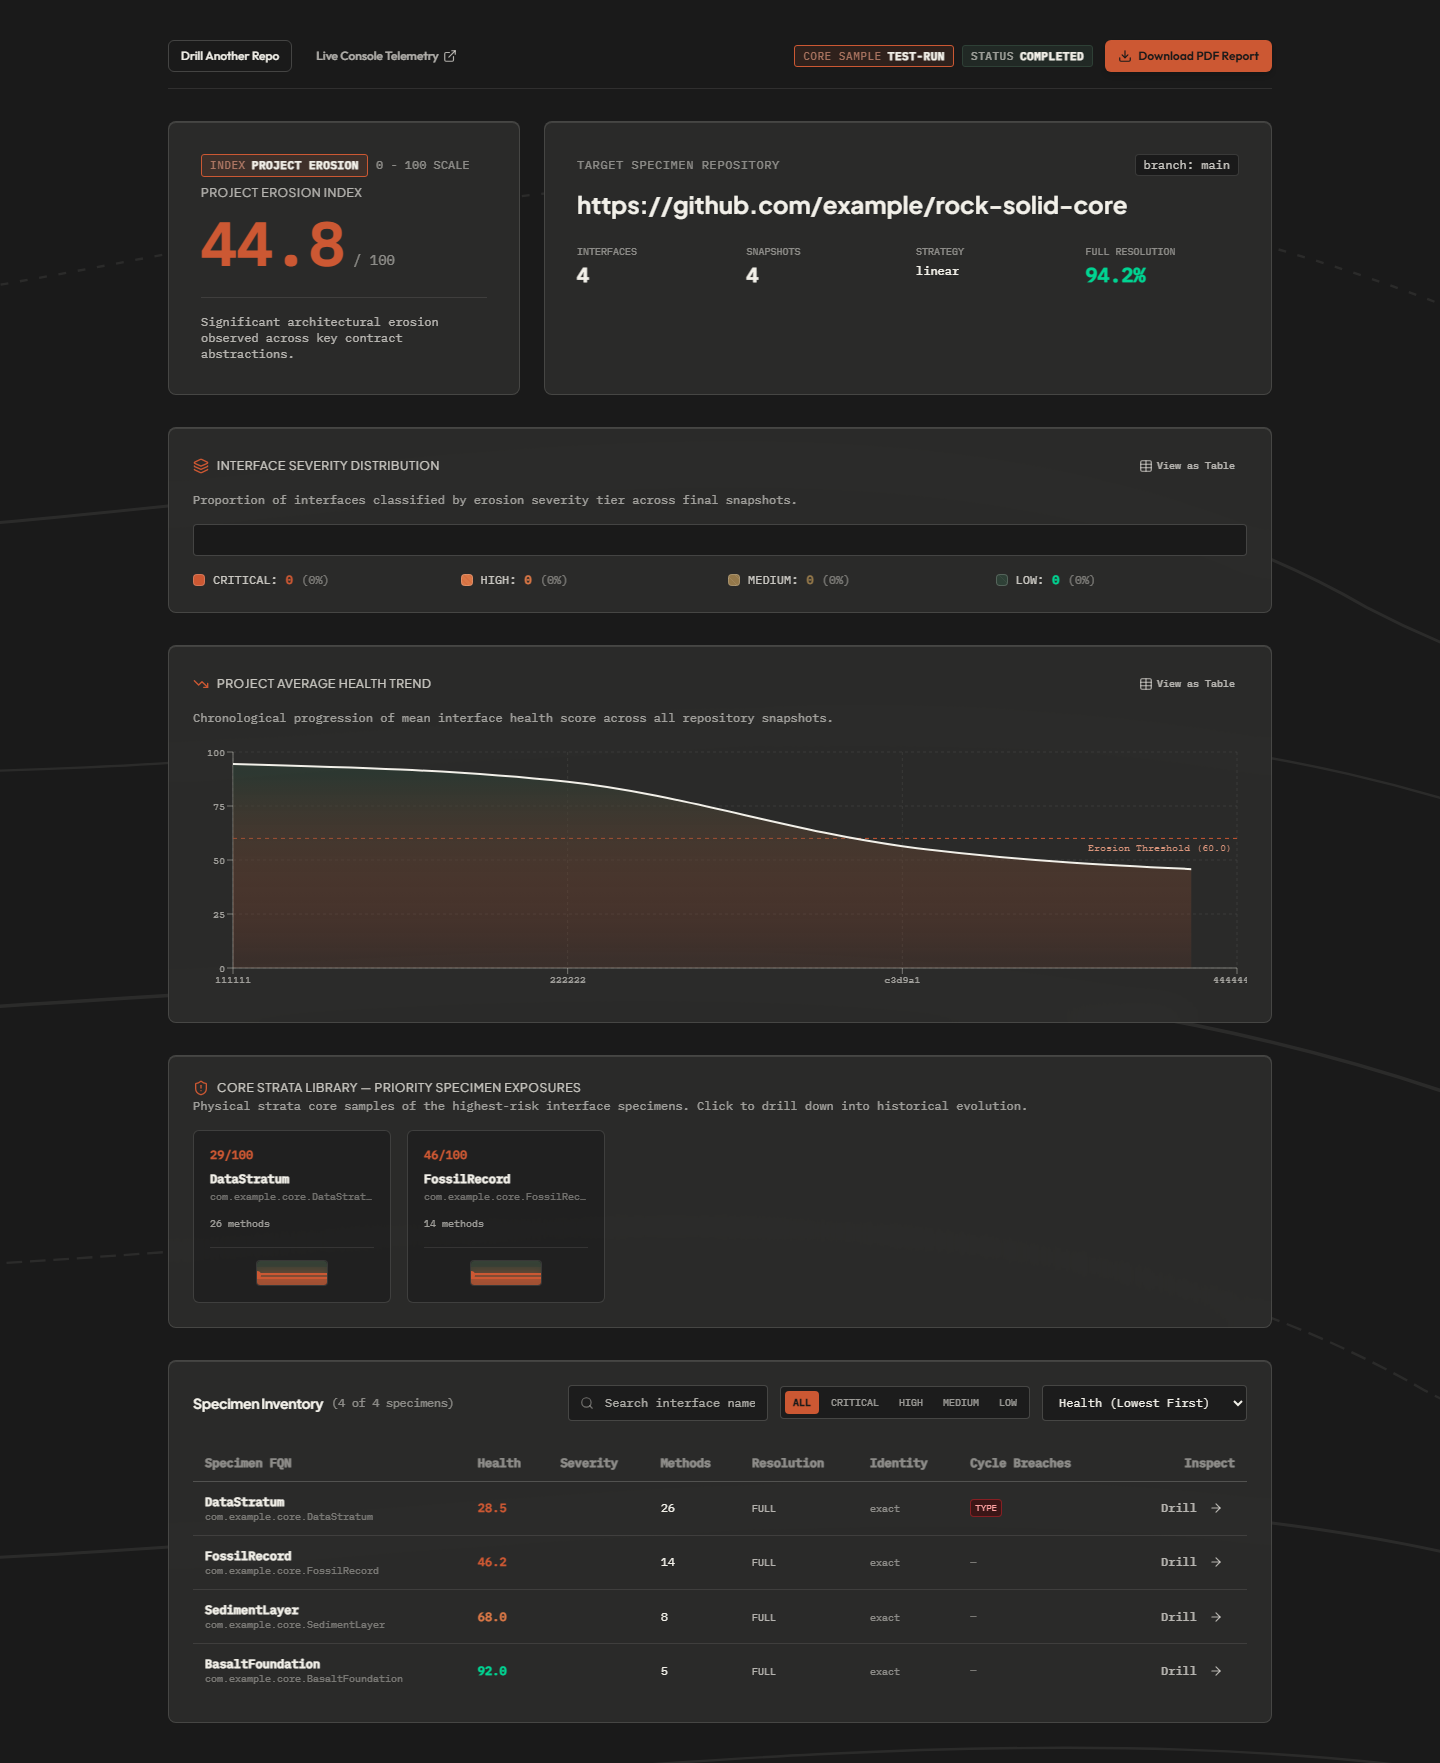
\includegraphics[width=0.92\textwidth]{screenshots/overview-1440px.png}%
}{%
  \fbox{\parbox[c][2.4in][c]{0.92\textwidth}{\centering\small Executive Architecture Overview Dashboard}}%
}
\caption{Executive Architecture Overview Dashboard with Health Scorecards}
\label{fig:screen_overview}
\end{figure}

\clearpage

\begin{figure}[H]
\centering
\IfFileExists{screenshots/specimen-1440px.png}{%
  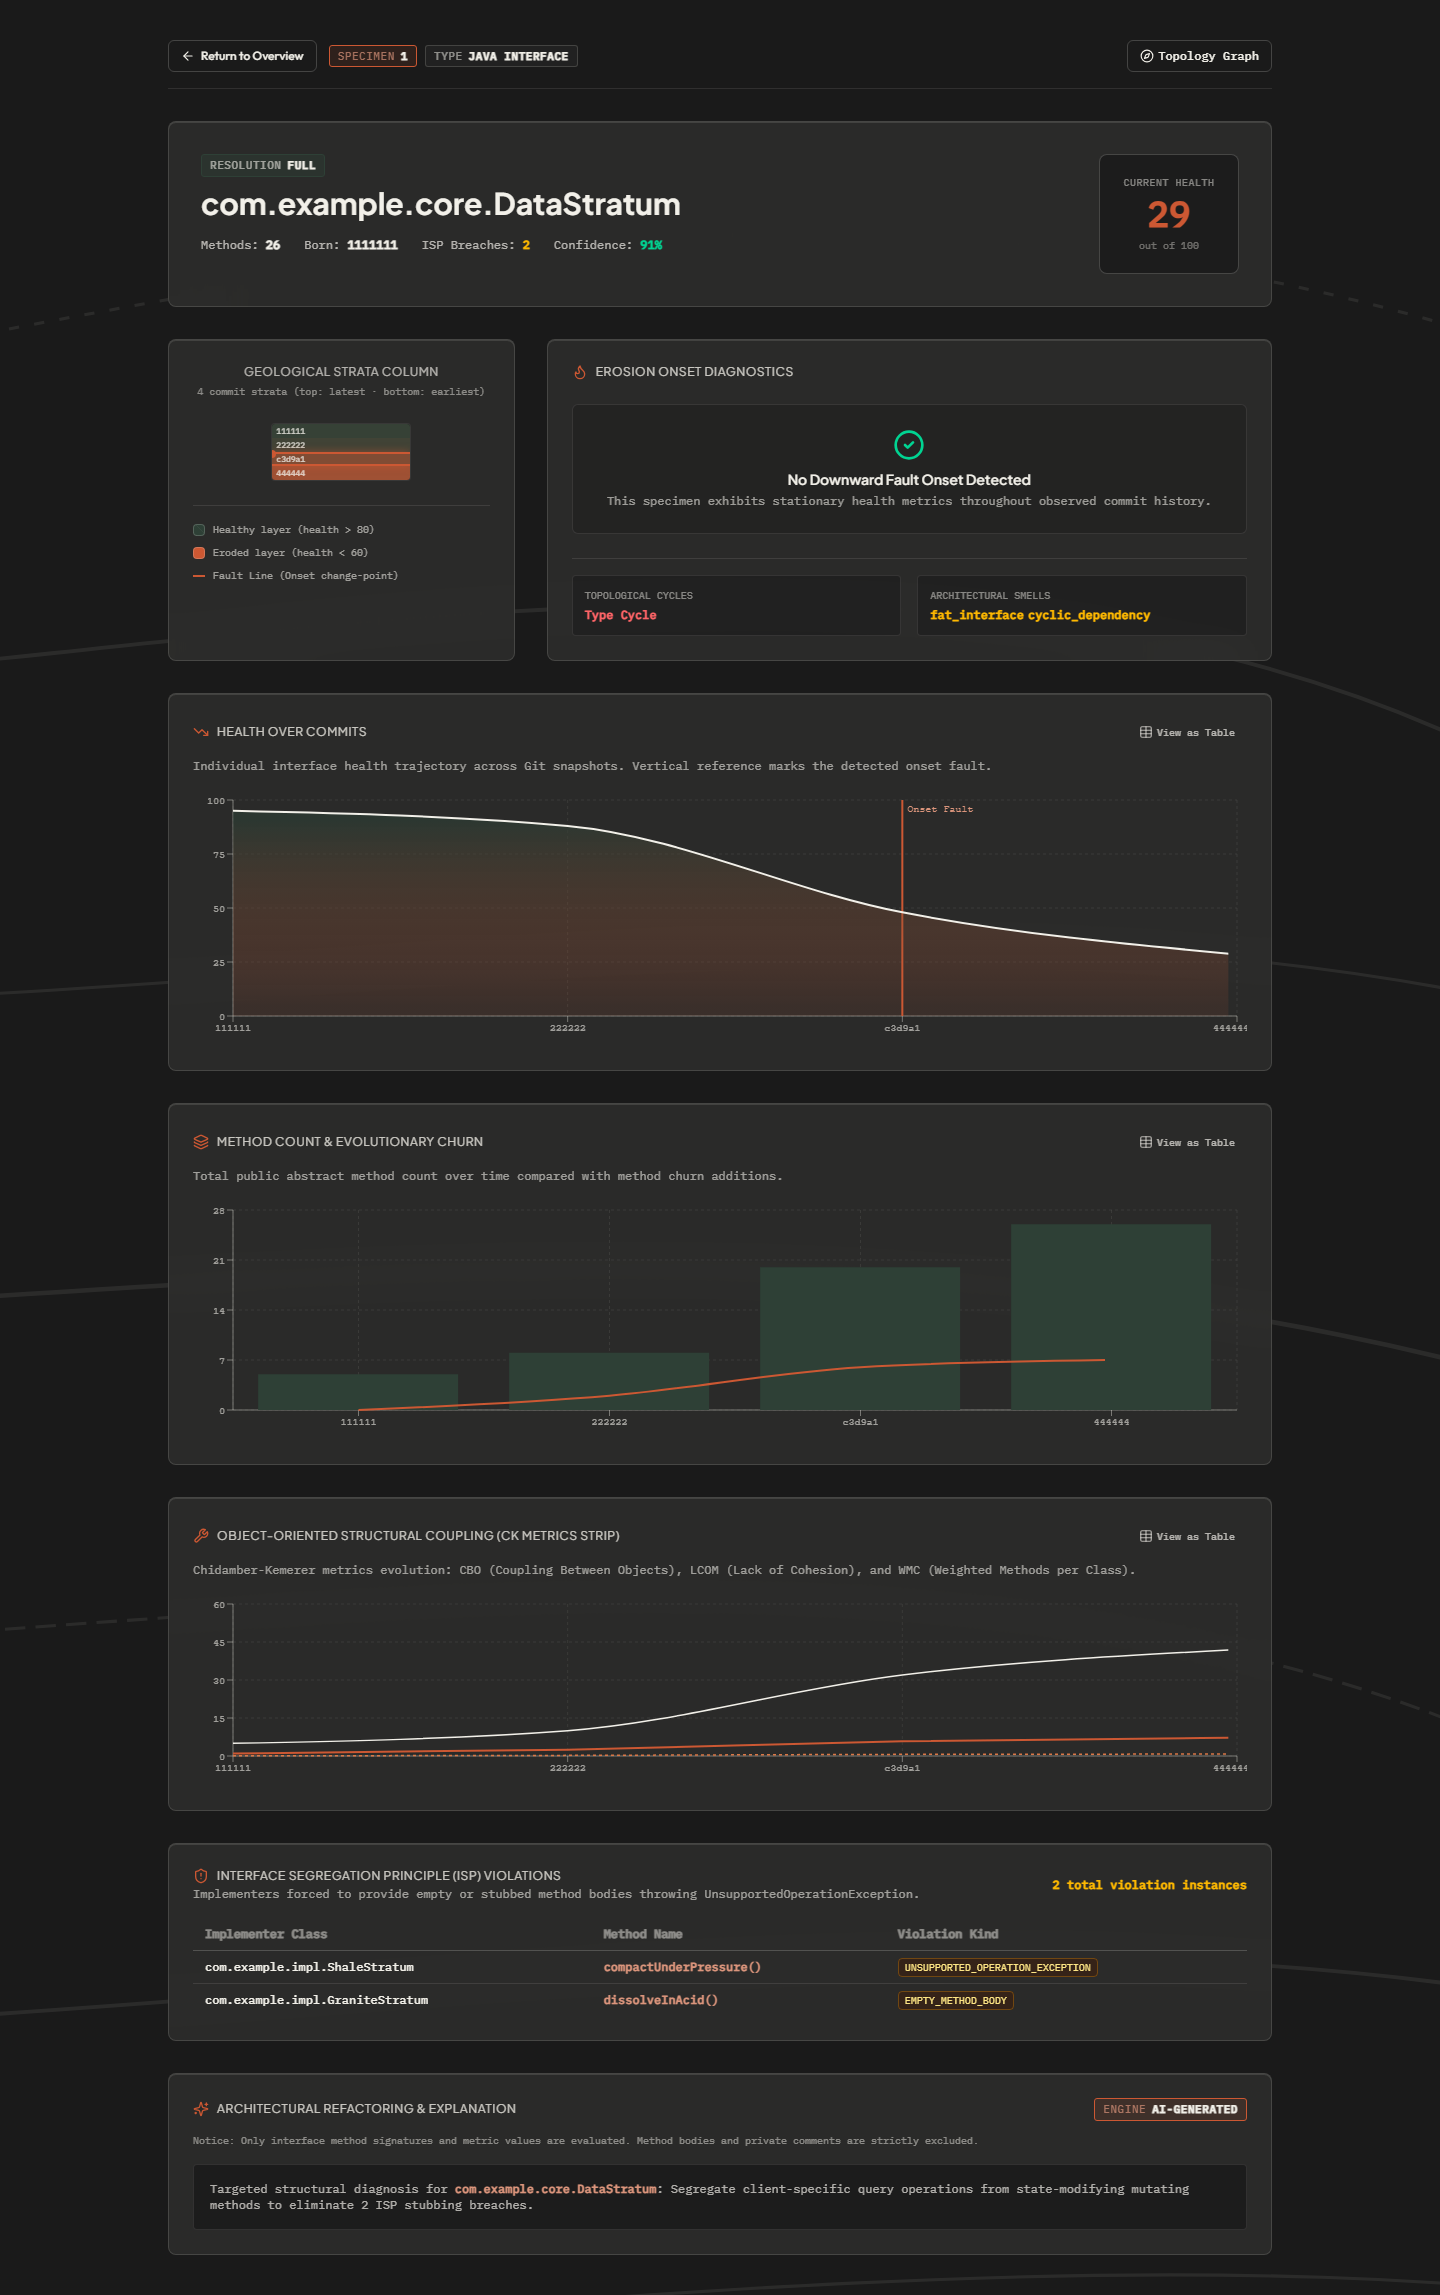
\includegraphics[width=0.92\textwidth]{screenshots/specimen-1440px.png}%
}{%
  \fbox{\parbox[c][2.4in][c]{0.92\textwidth}{\centering\small Interface Specimen Metric Inspector}}%
}
\caption{Interface Specimen Inspector with Historical Trend Breakdown}
\label{fig:screen_specimen}
\end{figure}

\begin{figure}[H]
\centering
\IfFileExists{screenshots/specimen-with-ai-1440px.png}{%
  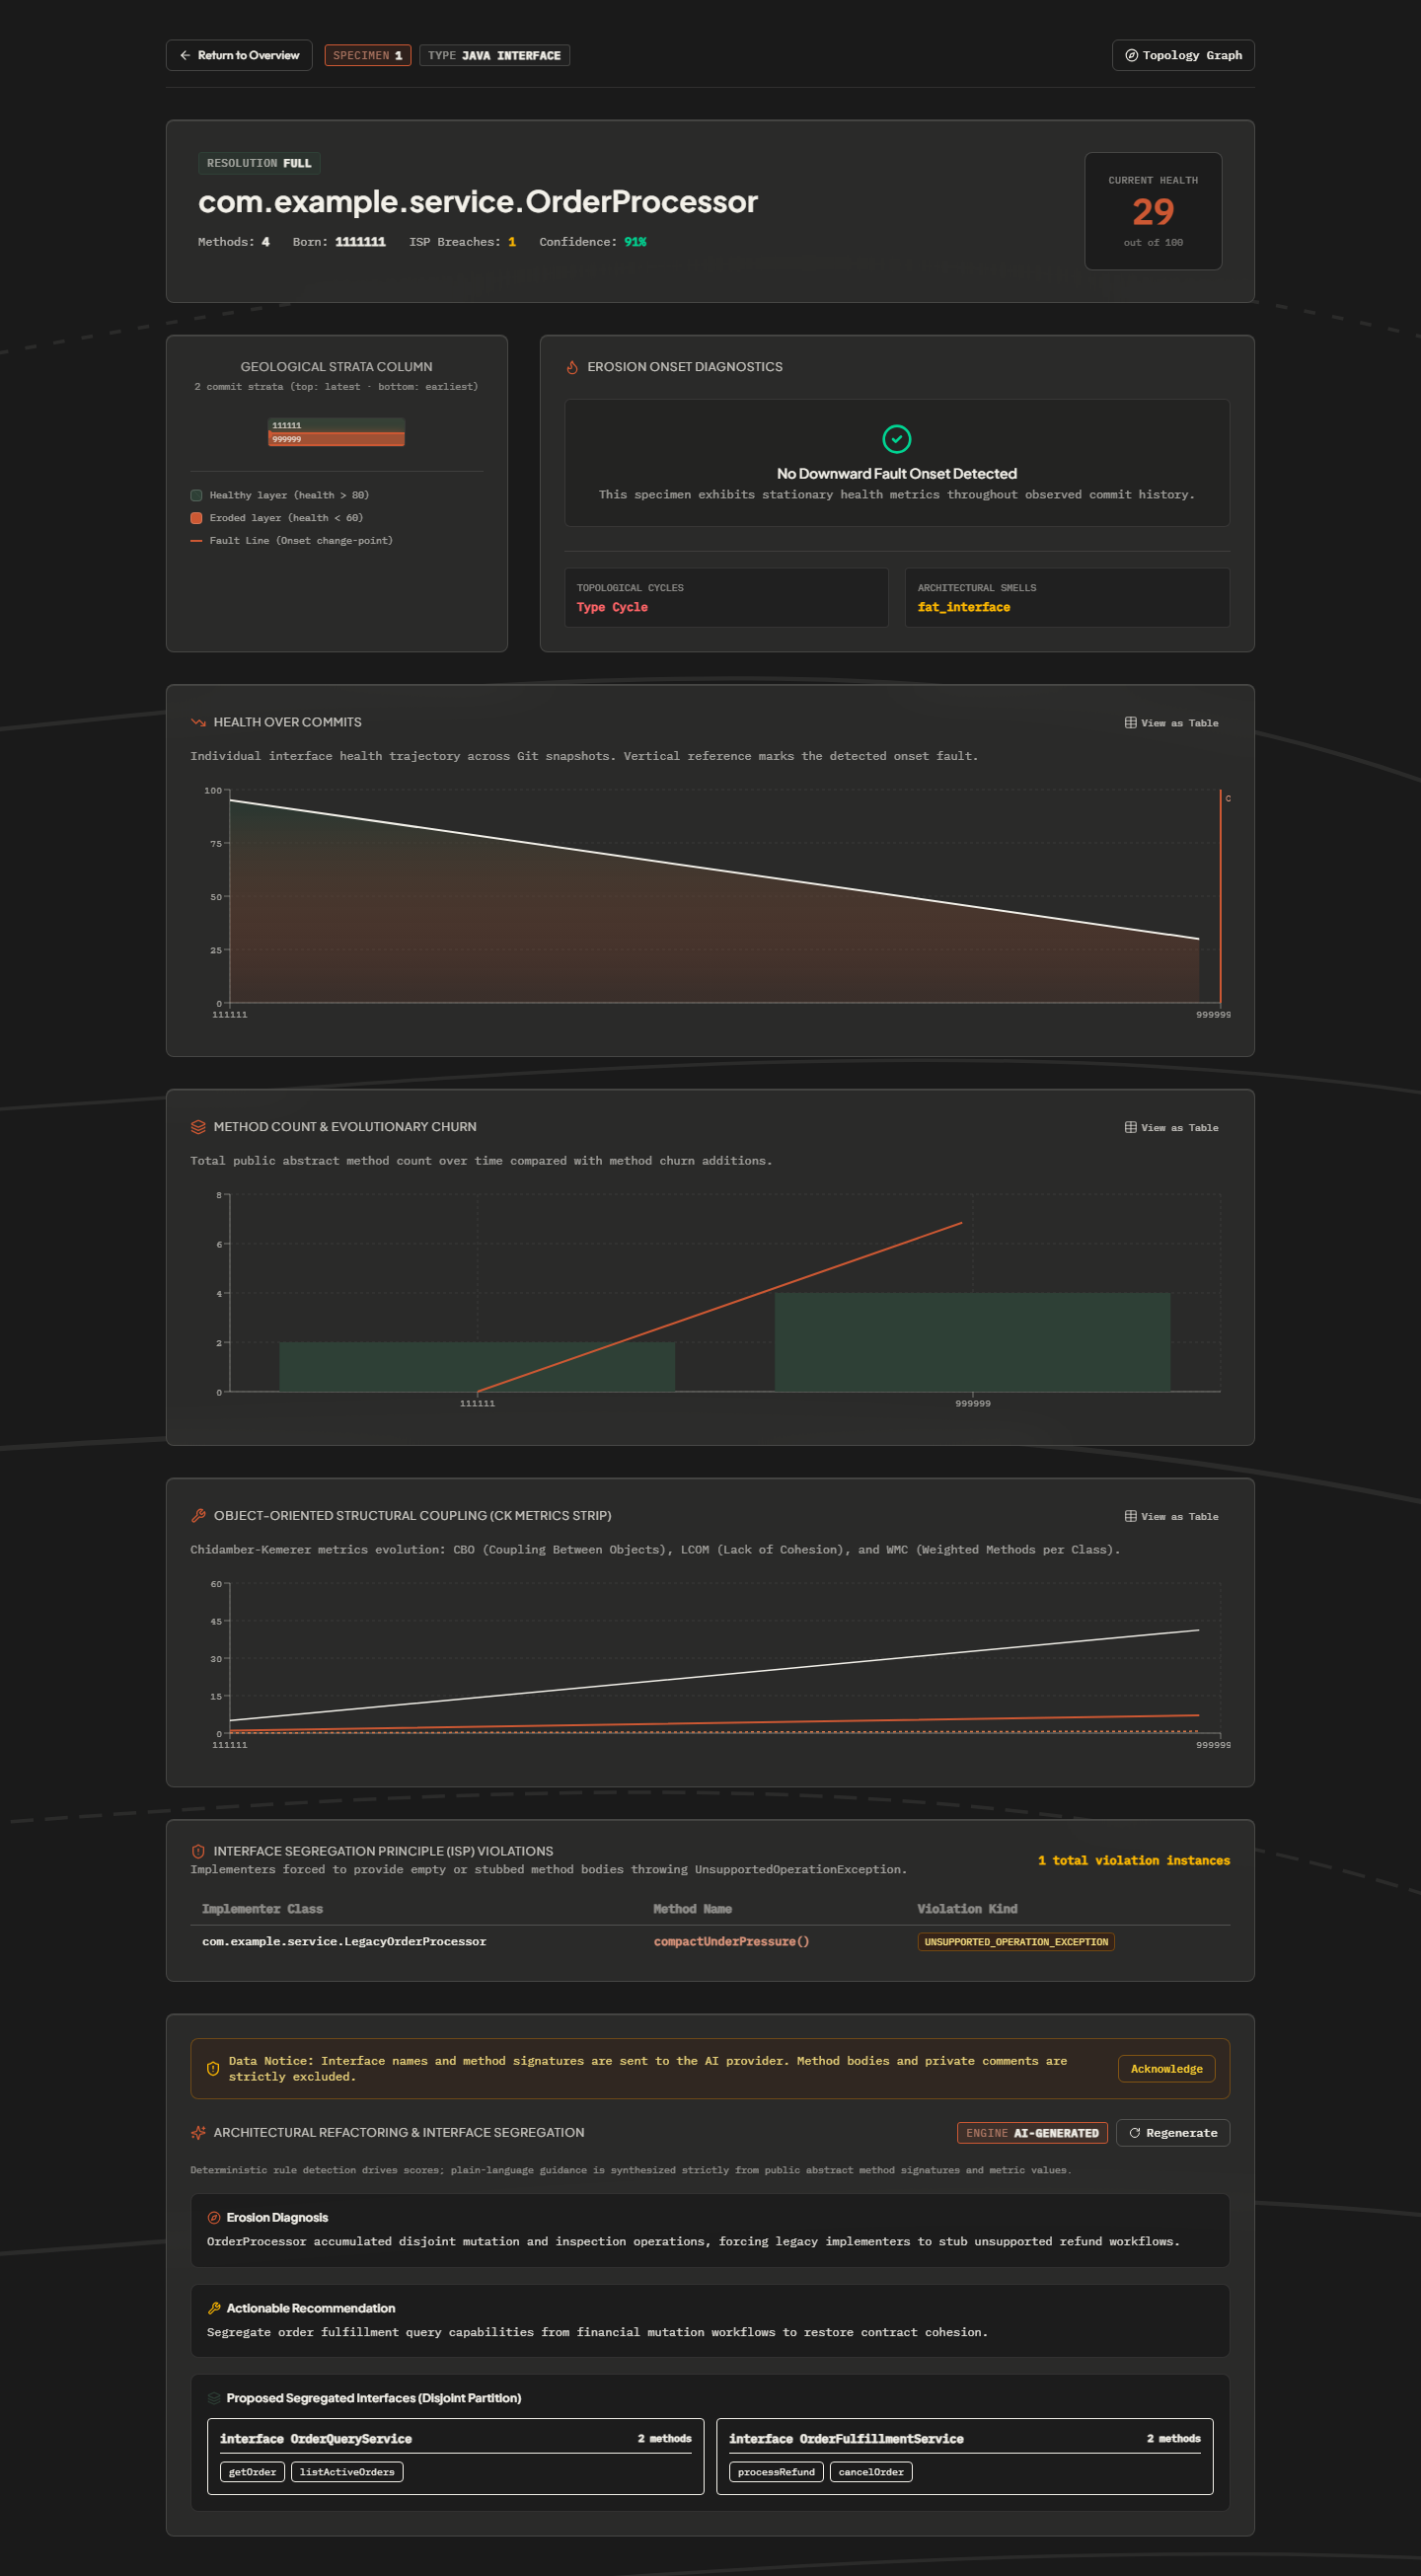
\includegraphics[width=0.92\textwidth]{screenshots/specimen-with-ai-1440px.png}%
}{%
  \fbox{\parbox[c][2.4in][c]{0.92\textwidth}{\centering\small AI Refactoring Guidance Drawer}}%
}
\caption{AI-Assisted Architectural Diagnostic and Separation-of-Concerns Advice}
\label{fig:screen_ai}
\end{figure}

\clearpage

\begin{figure}[H]
\centering
\IfFileExists{screenshots/graph-1440px.png}{%
  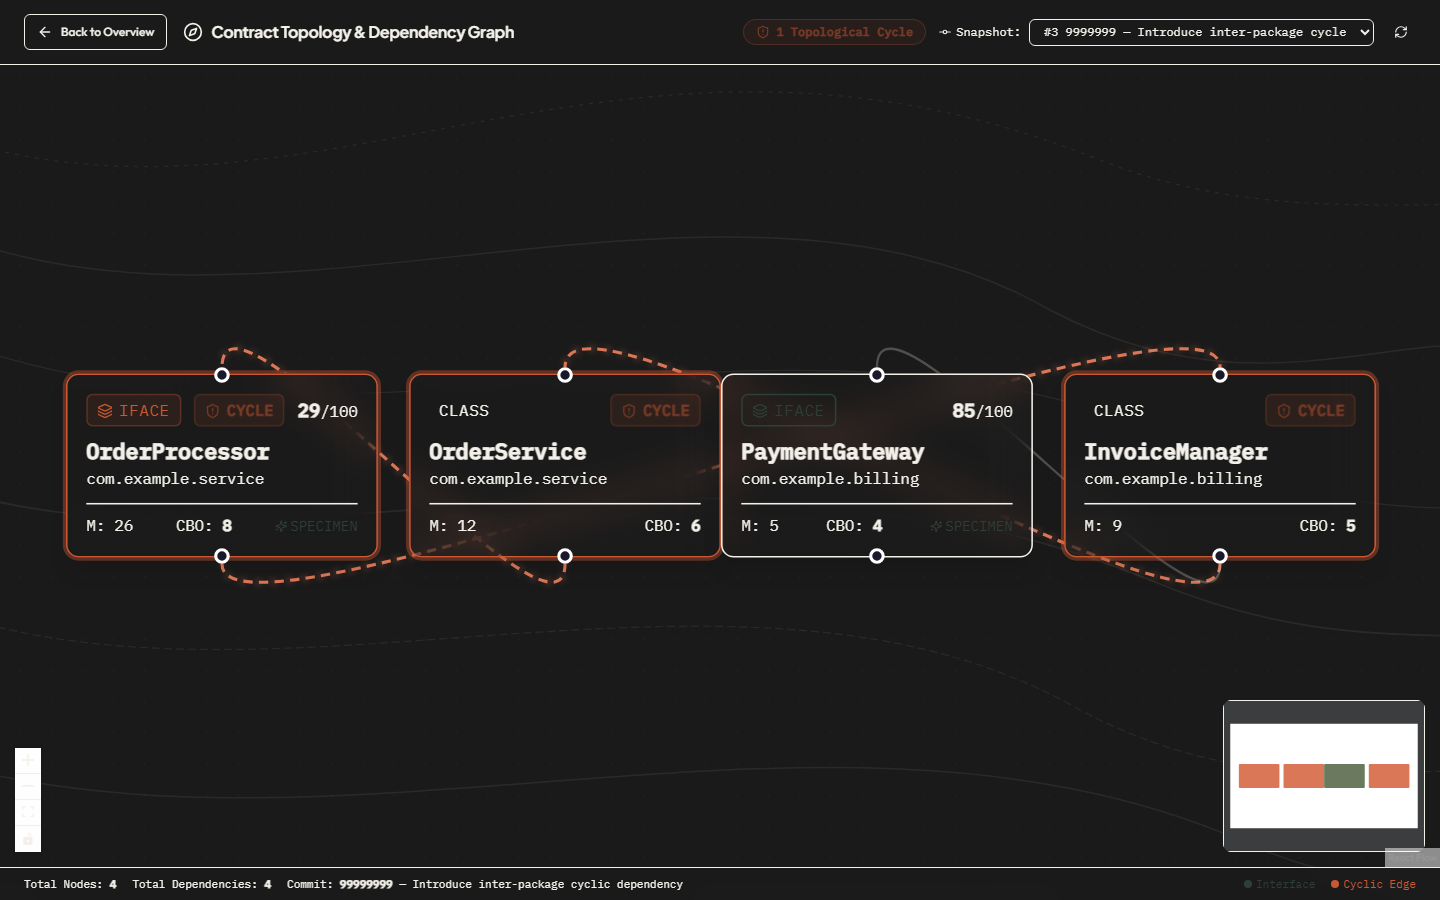
\includegraphics[width=0.92\textwidth]{screenshots/graph-1440px.png}%
}{%
  \fbox{\parbox[c][2.4in][c]{0.92\textwidth}{\centering\small Directed Dependency Graph View}}%
}
\caption{Interactive Directed Dependency Graph Built with React Flow}
\label{fig:screen_graph}
\end{figure}

\begin{figure}[H]
\centering
\IfFileExists{screenshots/graph-sidesheet-open.png}{%
  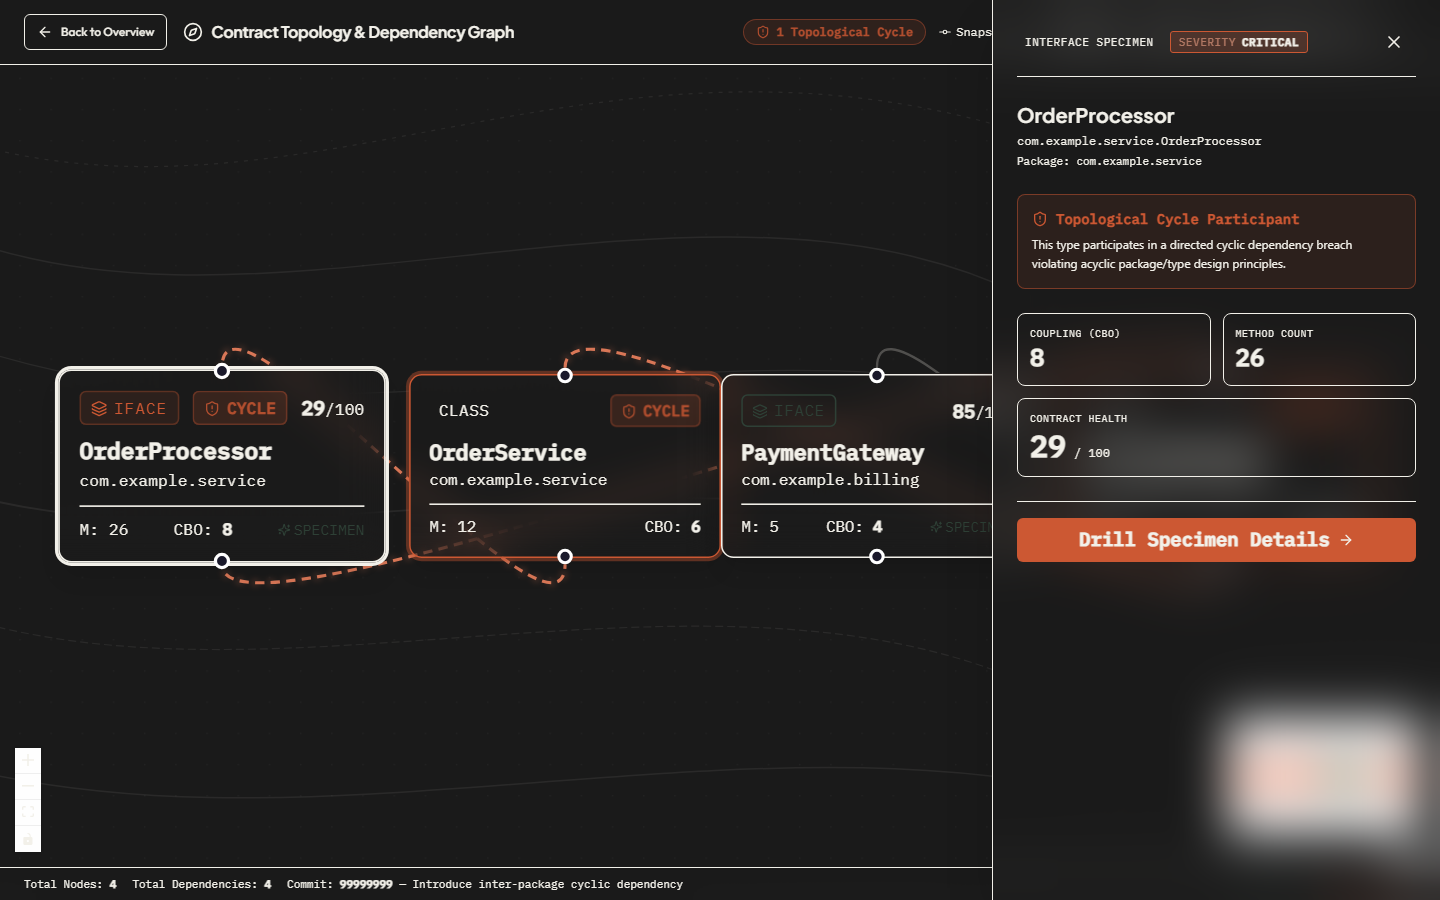
\includegraphics[width=0.92\textwidth]{screenshots/graph-sidesheet-open.png}%
}{%
  \fbox{\parbox[c][2.4in][c]{0.92\textwidth}{\centering\small Dependency Cycle Inspector Drawer}}%
}
\caption{Dependency Cycle Detection and Class Relationship Inspector Drawer}
\label{fig:screen_graph_side}
\end{figure}

\clearpage

\subsection{Burn Down Charts (Real Burndown Chart)}
\begin{spacing}{1.5}
\justifying
The project maintained consistent development velocity across all six sprints, completing all 83 planned story points without dropped features. Table~\ref{tab:sprint_hours} summarizes the sprint completion statistics, and Figure~\ref{fig:real_burndown} illustrates the real burndown trajectory.
\end{spacing}

\begin{table}[H]
\centering
\caption{Sprint-by-sprint completion metrics (Planned vs Actual)}
\label{tab:sprint_hours}
\renewcommand{\arraystretch}{1.4}
\setlength{\tabcolsep}{8pt}
\small
\begin{tabular}{|c|c|c|c|c|}
\hline
\textbf{Sprint} & \textbf{Planned Points} & \textbf{Completed Points} & \textbf{Remaining Points} & \textbf{Status} \\
\hline
Start & 83 & 0 & 83 & Baseline \\
\hline
Sprint 1 & 13 & 13 & 70 & Completed on schedule \\
\hline
Sprint 2 & 13 & 13 & 57 & Completed on schedule \\
\hline
Sprint 3 & 15 & 15 & 42 & Completed on schedule \\
\hline
Sprint 4 & 16 & 16 & 26 & Completed on schedule \\
\hline
Sprint 5 & 15 & 15 & 11 & Completed on schedule \\
\hline
Sprint 6 & 11 & 11 & 0 & Completed on schedule \\
\hline
\end{tabular}
\end{table}

\begin{figure}[H]
\centering
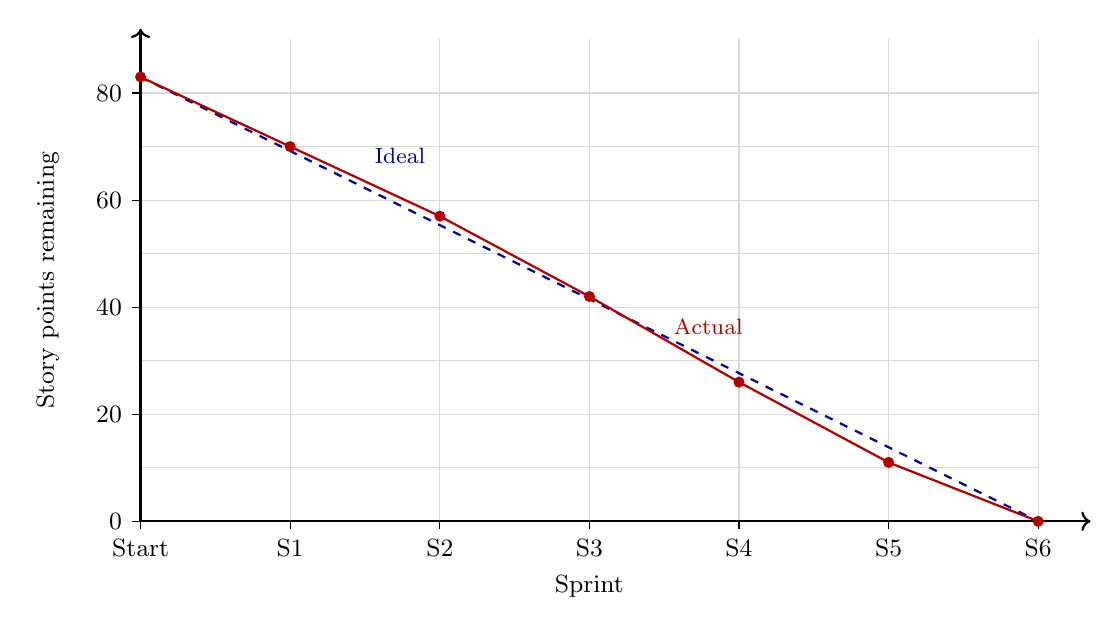
\begin{tikzpicture}[x=1.9cm,y=0.068cm,font=\small]
  \foreach \y in {10,20,...,80} \draw[gray!30] (0,\y) -- (6,\y);
  \foreach \x in {1,...,6} \draw[gray!30] (\x,0) -- (\x,90);
  \draw[->,thick] (0,0) -- (6.35,0);
  \draw[->,thick] (0,0) -- (0,92);
  \foreach \x/\l in {0/Start,1/S1,2/S2,3/S3,4/S4,5/S5,6/S6}
    \draw (\x,0) -- (\x,-1.5) node[below] {\l};
  \foreach \y in {0,20,40,60,80}
    \draw (0,\y) -- (-0.06,\y) node[left] {\y};
  \node[below=16pt] at (3,0) {Sprint};
  \node[rotate=90] at (-0.62,45) {Story points remaining};
  \draw[dashed,blue!60!black,thick] (0,83) -- (6,0);
  \draw[solid,red!70!black,thick] (0,83) -- (1,70) -- (2,57) -- (3,42) -- (4,26) -- (5,11) -- (6,0);
  \fill[red!70!black] (0,83) circle (2pt);
  \fill[red!70!black] (1,70) circle (2pt);
  \fill[red!70!black] (2,57) circle (2pt);
  \fill[red!70!black] (3,42) circle (2pt);
  \fill[red!70!black] (4,26) circle (2pt);
  \fill[red!70!black] (5,11) circle (2pt);
  \fill[red!70!black] (6,0) circle (2pt);
  \node[above right,blue!60!black] at (1.5,65) {\footnotesize Ideal};
  \node[above right,red!70!black] at (3.5,33) {\footnotesize Actual};
\end{tikzpicture}
\caption{Real burndown chart across six development sprints}
\label{fig:real_burndown}
\end{figure}

\clearpage

% ============================================================ 
% CHAPTER 12: REFERENCES/BIBLIOGRAPHY
% ============================================================ 
\section{REFERENCES/BIBLIOGRAPHY}

\begin{spacing}{1.5}
\justifying
\textbf{Books and Articles:}
\begin{enumerate}[leftmargin=*,itemsep=2pt]
  \item Martin, R. C. (2002). \textit{Agile Software Development, Principles, Patterns, and Practices}. Prentice Hall.
  \item Fowler, M. (2018). \textit{Refactoring: Improving the Design of Existing Code} (2nd ed.). Addison-Wesley Professional.
  \item Gamma, E., Helm, R., Johnson, R., \& Vlissides, J. (1994). \textit{Design Patterns: Elements of Reusable Object-Oriented Software}. Addison-Wesley.
  \item Sommerville, I. (2016). \textit{Software Engineering} (10th ed.). Pearson Education.
\end{enumerate}

\textbf{Research Papers:}
\begin{enumerate}[leftmargin=*,itemsep=2pt]
  \item Chidamber, S. R., \& Kemerer, C. F. (1994). A metrics suite for object oriented design. \textit{IEEE Transactions on Software Engineering}, 20(6), 476--493.
  \item Page, E. S. (1954). Continuous inspection schemes. \textit{Biometrika}, 41(1/2), 100--115.
  \item Spadini, D., Aniche, M., \& Bacchelli, A. (2018). PyDriller: Python framework for mining software repositories. \textit{Proceedings of ESEC/FSE}, 900--903.
  \item Truong, C., Runge, L., \& Bleakley, K. (2020). Selective review of offline change point detection methods. \textit{Signal Processing}, 174, 107619.
\end{enumerate}

\textbf{Websites and Technical Documentation:}
\begin{enumerate}[leftmargin=*,itemsep=2pt]
  \item JavaParser Documentation: \url{https://javaparser.org}
  \item PyDriller Documentation: \url{https://pydriller.readthedocs.io}
  \item Flask Framework: \url{https://flask.palletsprojects.com}
  \item React Official Guide: \url{https://react.dev}
  \item NetworkX Graph Library: \url{https://networkx.org}
  \item WeasyPrint Documentation: \url{https://weasyprint.org}
\end{enumerate}

\textbf{Standards and Guidelines:}
\begin{enumerate}[leftmargin=*,itemsep=2pt]
  \item IEEE Std 1074-2006: IEEE Standard for Developing Software Life Cycle Processes.
  \item ISO/IEC 25010: Systems and Software Engineering --- Quality Models.
  \item PEP 8: Style Guide for Python Code. Python Software Foundation.
\end{enumerate}
\end{spacing}

\end{document}